\section{Die Algorithmen auf diesem Markt}
Der Vergleich der RL-Algorithmen findet auf dem in \ref{section:markov} definierten Markt statt.
Dieser Markt wird auf der Testplattform simuliert, die im Rahmen des Bachelorprojektes entwickelt wurde.
Mit den Agenten wird über die Gym-Schnittstelle kommuniziert. \cite{brockman2016openai}
Für die zu vergleichenden Algorithmen werden die Implementierungen der Bibliothek \textit{Stable Baselines} verwendet. \cite{stable-baselines}
Stable Baselines ist eine weit verbreitete eine Open-Source RL-Bibliothek, die in Python geschrieben ist.
Sie baut auf PyTorch auf, einem der beliebtesten Deep-Learning-Frameworks, das in der Forschung weite Verbreitung findet. \cite{NEURIPS2019_9015}
Die in Stable Baselines implementierten Algorithmen entsprechen in den meisten Fällen unmittelbar den vorgeschlagenen Algorithmen der Originalpaper und zeichnen sich durch eine hohe Lesbarkeit des Codes aus. \footnote{Die SAC-Implementierung verwendet nicht den Reparameterization Trick}
Alle Hyperparameter sind konfigurierbar.

Weil kaum theoretische Erkenntnisse über die Ermittlung optimaler Hyperparameter vorliegen und diese stets problemspezifisch sind, wäre eine erschöpfende Optimierung der Hyperparameter nur mit erheblichem experimentellem Aufwand möglich.
Das ist nicht im Umfang dieser Arbeit.
In dieser Untersuchung der Algorithmen wird deshalb von den Hyperparametern der Originalpaper ausgegangen.
Diese sind auch im Abschnitt \ref{section:hyperparameter} zu finden.
Dennoch wurden an einigen Stellen bessere Hyperparameter gefunden und Aussagen über die Algorithmen über mehrere Hyperparameterkombinationen abgesichert.

Alle Verfahren werden mit neuronalen Netzen durchgeführt, die zwei versteckte Schichten mit je 64 Neuronen haben.
%Das Verhalten der Algorithmen für unterschiedliche Netzgrößen ist aber sehr ähnlich, wie die Experimente mit unterschiedlichen Netzgrößen im Bereich [noch zu erstellen] des Anhangs zeigen.
Zunächst werden alle Algorithmen im Duopol gegen den regelbasierten, unterbietenden Wettbewerber aus Abschnitt \ref{section:rulebased_definition} trainiert und evaluiert.
Anschließend werden Training gegen die eigene Policy, unvollständige Informationen, angepasste Rewardfunktion und Monopol- und Oligopolszenarien untersucht.

\section{DDPG und TD3}
\label{section:main_ddpg}
Bei der Diskussion der Q-Learning-Verfahren beschränkt sich diese Analyse direkt auf die Verfahren, die im stetigen Raum angewendet werden: DDPG und TD3.
Diese Beschränkung wird gemacht, weil in den diskutierten vorherigen Analysen zu Pricing Verfahren mit diskretem Aktionsraum weniger erfolgreich waren als solche mit stetigem Aktionsraum.
Der Hauptgrund allerdings, der das Verfahren mit diskretem Aktionsraum für diese Arbeit ausschließt, ist, dass Deep-Q-Networks mit diskreten Aktionen jede einelnen Aktionen aus $\mathcal{A_\mathbb{N}}$ mit einem Aktionswert versehen müssten.
Das sind bei der Konfiguration mit $p_{max}=10$ bereits 1000 Ausgabeneuronen und das Wachstumsverhalten ist kubisch in der Anzahl der Preisstufen.

\begin{figure}[htbp]
	\centering
	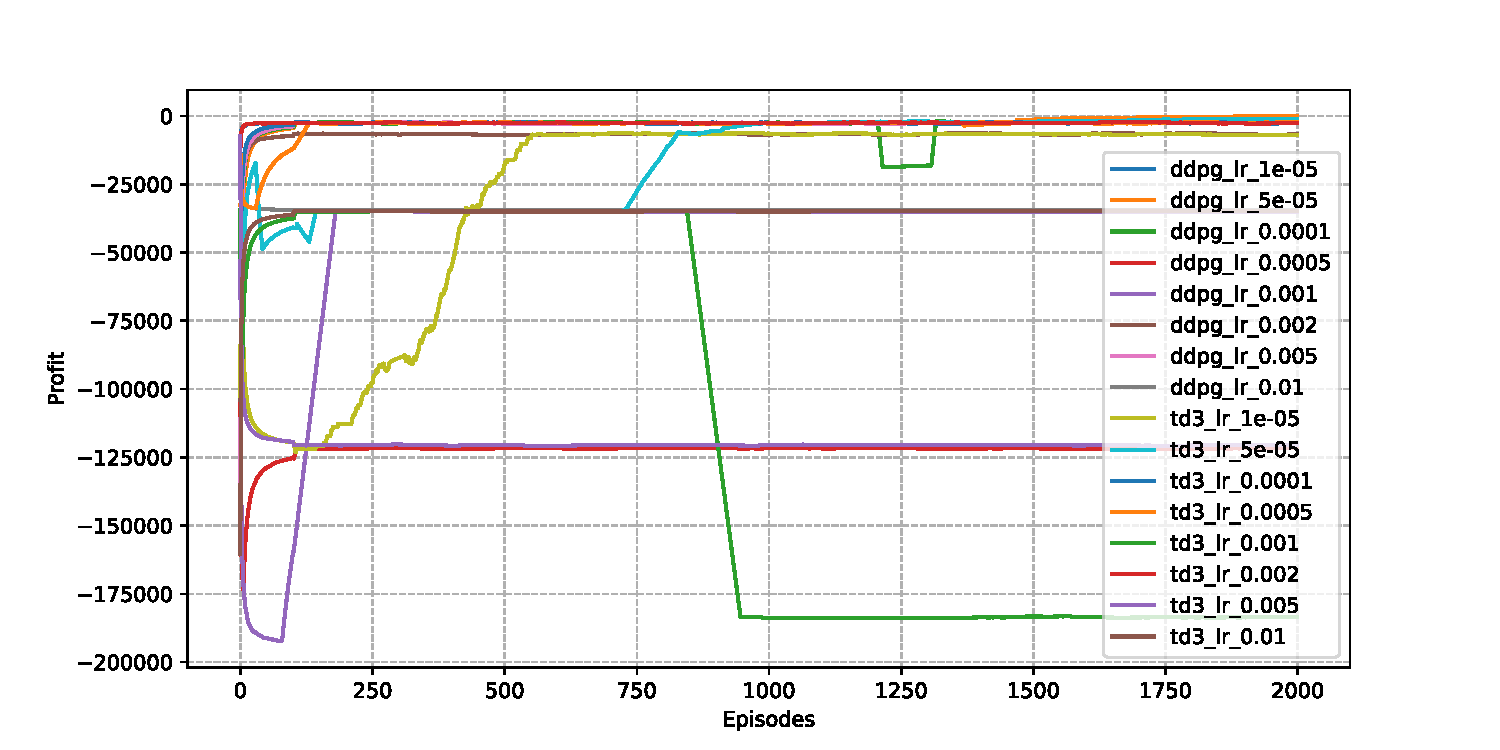
\includegraphics[width=\textwidth]{main/ddpg_td3.pdf}
	\caption{Lernkurven von DDPG und TD3 mit unterschiedlichen Lernraten}
	\label{graphic:DDPGLearningCurve}
\end{figure}

Die Lernkurven der beiden sehr ähnlichen Verfahren DDPG und TD3 sind in Abbildung \ref{graphic:DDPGLearningCurve} dargestellt.
Für jeden der beiden Algorithmen wurden acht Trainingsläufe durchgeführt, die mit unterschiedlichen Lernraten parametrisiert wurden.
Der Standardwert liegt für beide Algorithmen bei $10^{-3}$.
Es wurden Trainingsläufe mit diesen Lernraten sowie kleineren und größeren durchgeführt.
Die beim Training beobachteten Muster gleichen sich sowohl bei den beiden Algorithmen als auch den unterschiedlichen Parametrisierungen.

Zu Beginn des Trainings ist bei einigen Läufen eine Verbesserung der gemittelten Returns, die primäre Leistungskennziffer, zu beobachten.
Allerdings kommt diese Verbesserung bei allen Algorithmen zum Erliegen, keiner erwirtschaftet Gewinne.

Die schlechten Ergebnisse kommen deshalb zustande, weil über das gesamte Training hinweg nicht lernen, die Preise vernünftig zu setzen.
Bei vielen Durchläufen bleiben die Neupreise ohne Anpassung auf die aktuelle Situation beim Maximum 10 hängen, oft sogar auch die Gebrauchtpreise.
Die Tatsache, dass die Agenten lange auf einer Stelle bleibt und auch die gleichen verbesserungswürdigen Aktionen immer wieder ausführt, könnte auf unzureichende Exploration schließen lassen.
Allerdings konnte auch eine verrauschte Aktionswahl zur besseren Exploration keine Verbesserung der Leistung erreichen.

Weiterhin sieht man in den Trainingsdurchläufen, dass sich die Leistung oft ruckartig verändern.
Der dabei in den Lernkurven zu erkennende lineare Auf- oder Abstieg ist der Durchschnittsbildung über die letzten hundert Episoden geschuldet.
Tatsächlich findet die Änderung sprunghaft statt.

Zahlreiche der Trainingsdurchläufe sind von starken Einbrüchen der Leistung geprägt.
Obwohl Instabilität bei DDPG und TD3 als Probleme bekannt sind, enttäuscht, dass trotz verschiedenster ausprobierter Werte in der Lernrate und Techniken zur verstärkten Exploration die Beherrschung dieses Marktes nicht erlernt werden konnte.
Deshalb werden in den folgenden Abschnitten DDPG und TD3 nicht weiter betrachtet.

\section{On-Policy-Learning -- A2C und PPO}
\label{section:main_ppo}
Die beiden On-Policy-Verfahren A2C und PPO gibt es für diskrete wie für stetige Aktionsräume.
Wegen der großen Zahl der Aktionen wird auch hier jedoch nur die stetige Variante ausprobiert.

\begin{figure}[htbp]
	\centering
	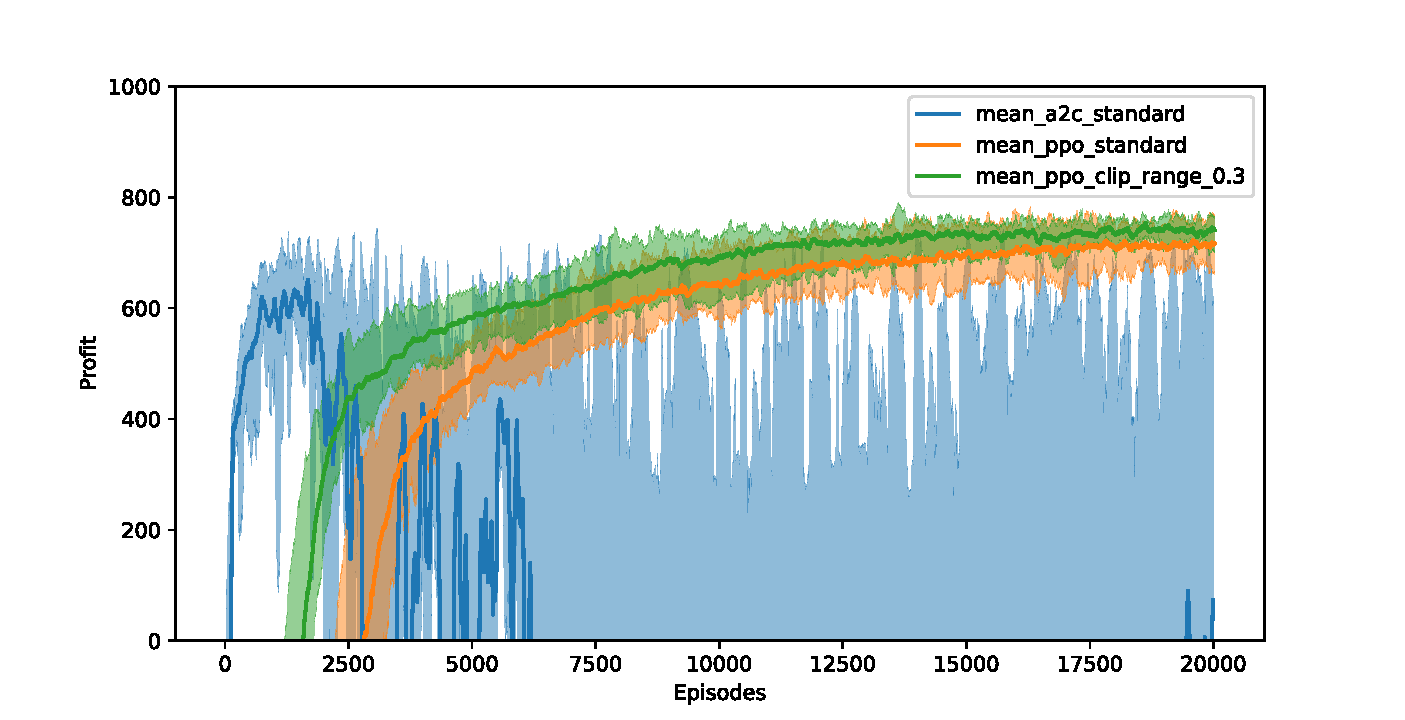
\includegraphics[width=\textwidth]{main/a2c_vs_ppo.pdf}
	\caption{Lernkurven von A2C und PPO auf dem Duopol mit unterbietendem Wettbewerber}
	\label{graphic:OnPolicyLearningCurves}
\end{figure}

Grafik \ref{graphic:OnPolicyLearningCurves} stellt die Lernkurven der Algorithmen dar.
Dabei wurde PPO mit zwei Hyperparametrisierungen verwendet, die sich im Parameter $\epsilon$ unterscheiden.
Das eine Mal wird $0.2$ wie im Originalpaper verwendet, das andere Mal $0.3$.
Jedes dieser Experimente wurde vier Mal unabhängig für eine Million Schritte (zweitausen Episoden) laufen gelassen.
Die Lernkurven verwenden wieder die laufenden Durchschnitte der Episodenreturns.
Der Bereich zwischen maximalem und minimalem Episodenreturns dieser vier Agenten ist eingefärbt.
Die Linie stellt ihren Durchschnitt dar.
In dieser Grafik wird der Verlustbereich ausgeblendet, um einen genaueren Vergleich im oberen Leistungsbereich zu ermöglichen.

Aus den Grafiken geht unmittelbar hervor, dass alle diese Agenten die Gewinnzone erreichen.
Sie erreichen alle mit Ergebnissen über 6000 pro Episode gute Ergebnisse.
Auf Grundlage dieser Grafik kann man feststellen, dass die Parametrisierung mit $\varepsilon=0.3$ bessere Performance einbringt als die Standardparametrisierung.
Um die Spitzenperformance vergleichen zu können, sind die Lernkurven jedoch nur bedingt geeignet.

Für konkrete Aussagen über die Spitzenperformance wurde bei jedem Trainingsdurchlauf alle 100 Episoden das nach dem rolling Average beste Modell aus den vorigen 100 Episoden gespeichert.
Nach dem Training wurden diese Modelle auf je 25 unabhängigen Episoden getestet, um eine genauere Schätzung ihrer Performance zu erhalten.
Die Spitzenwerte der drei A2C-Trainingsdurchläufe lagen bei 8160, 8520, 7150 und 8510.
Bei den PPO-Durchläufen mit $\varepsilon=0.2$ waren die Spitzenwerte 7380, 7780, 8330 und 8120.
Die PPO-Durchläufe mit $\varepsilon=0.3$ erreichten 8300, 8680, 8360 und 8350.
Dass die Spitzen der A2C-Durchläufe in der Lernkurve niedriger sind als die hier aufgeführten Spitzenwerte, liegt an den rolling Averages und der erheblich geringeren Trainingsstabilität der A2C-Agenten.
Sie halten das hohe Leistungsniveau nur sehr kurz, weshalb die Mittelwertbildung mit anderen Ergebnissen während des Trainings niedrigere Werte ergibt.
Sichert man jedoch die Parameter der Modelle, wenn sie gerade gute Ergebnisse liefern, erhält man wettbewerbsfähige Leistung.

Die Advantage-Actor-Critic-Agenten erreichen das hohe Leistungsniveau dabei nach deutlich weniger Episoden als die PPO-Agenten.
Ihr Durchschnitt überschreitet die Schwelle zum Gewinn nach etwa 70 Episoden (3500 Schritten).
\begin{figure}[htbp]
	\centering
	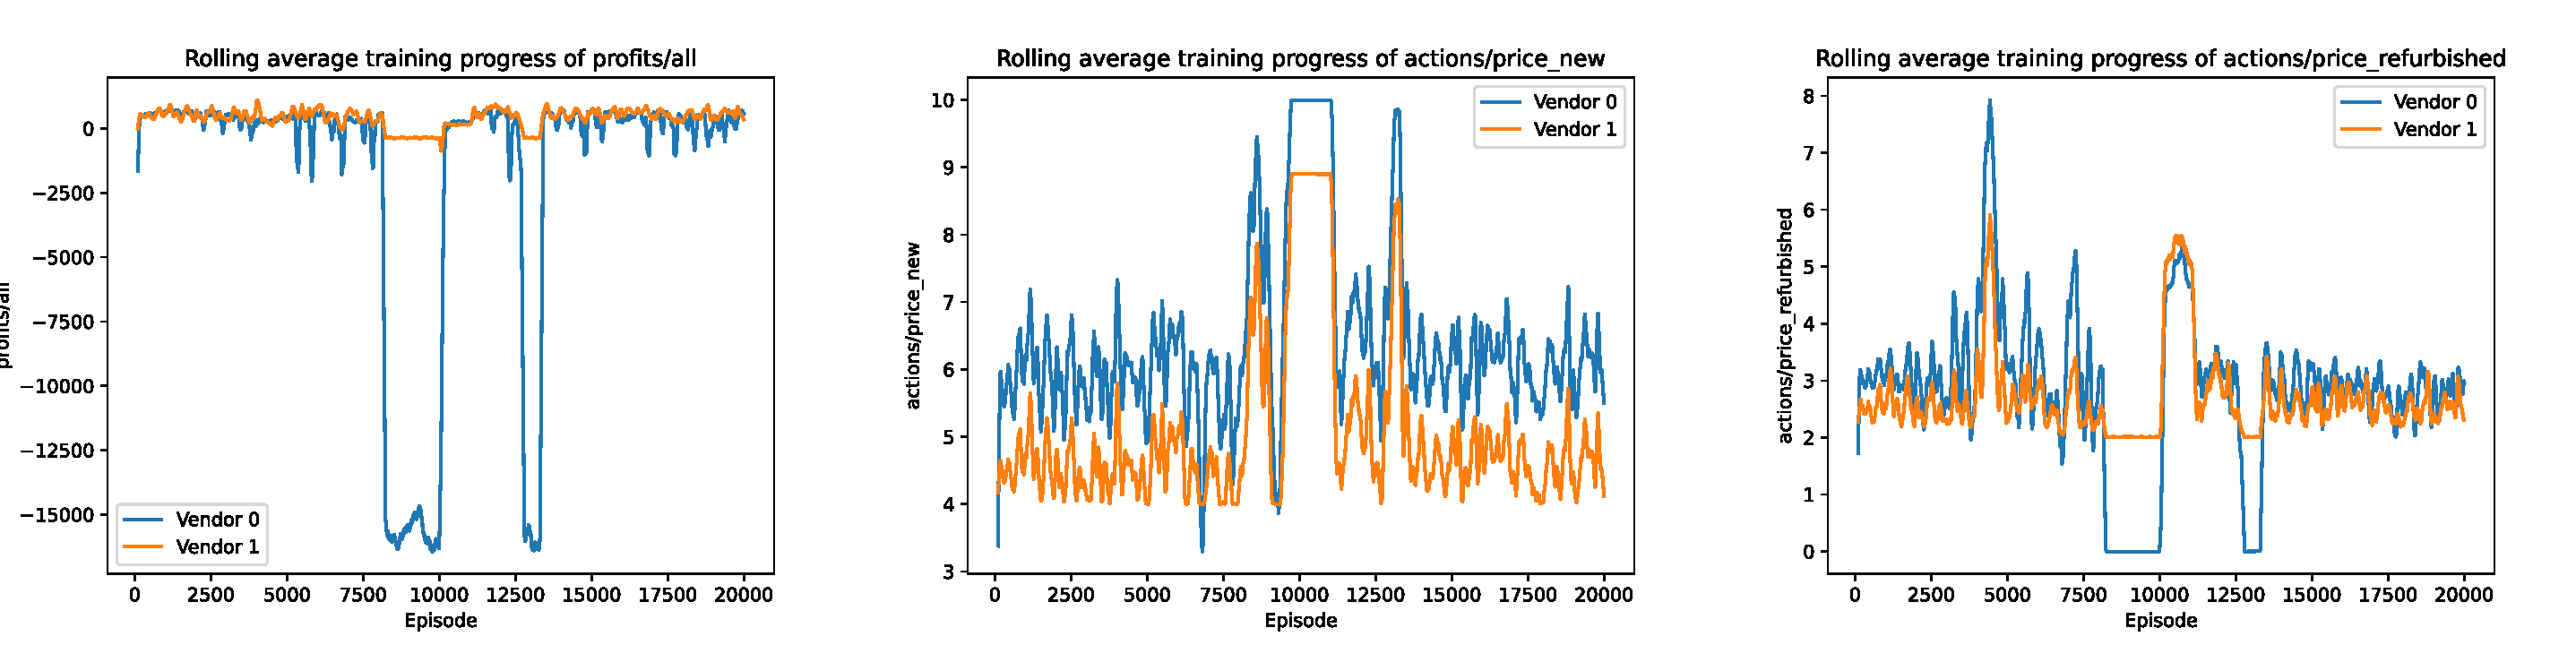
\includegraphics[width=\textwidth]{main/a2c_detailed_analysis.pdf}
	\caption{
		Detaillierte Betrachtung eines A2C-Trainingsdurchlaufes zur Visualisierung der Instabilität, wobei Vendor\_0 der RL-Agent und Vendor\_1 der regelbasierte, direkte Wettbewerber während des Trainings ist:
		(links) Lernkurve mit schnellem initialem Anstieg, danach Abstürze und Erholungen;
		(mitte) durchschnittliche Auswahl der Neupreise, zeigt erhebliche Schwankungen;
		(rechts) durchschnittliche Auswahl der Gebrauchtpreise, ebenfalls instabil
	}
	\label{graphic:A2CInstability}
\end{figure}
Die Grafik \ref{graphic:A2CInstability} stellt Details eines einzelnen A2C-Durchlaufes dar.
Es handelt sich dabei um einen typischen Durchlauf mit mittlerer Peak-Performance.
Man sieht die Instabilität nicht nur an den Ergebnissen sondern auch an den starken Schwankungen, denen die Aktionsauswahl während des Trainings unterworfen ist.
Wie auch bei den anderen A2C-Agenten stürzt seine Leistung mitunter deutlich ab und fällt dabei weit in die Verlustzone.
Nicht immer erholen sich die Agenten davon, oft erhalten sie weiterhin schlechte Ergebnisse.
Diese heftigen Abstürze führen dazu, dass die Mittelwertlinie der A2C-Agenten in Abbildung \ref{graphic:OnPolicyLearningCurves} wieder unter 0 fällt, obwohl einige der Agenten weiterhin akzeptable Ergebnisse liefern.

Im Gegenzug dazu ist die Trainingsstabilität bei den PPO-Varianten deutlich höher.
Zwischen den vier Trainingsdurchläufen der PPO-Agenten gibt es nur geringe Unterschiede.
Die Leistungsentwicklung liegt in einem schmalen Band und Abstürze finden nicht statt.
Allerdings benötigt PPO in der Standardkonfiguration knapp 250 Episoden und in der Version mit $0.3$ als $\varepsilon$ ungefähr 180 Episoden, um die Gewinnzone zu erreichen.
Auch danach ist das Training langsam.
\begin{figure}[htbp]
	\centering
	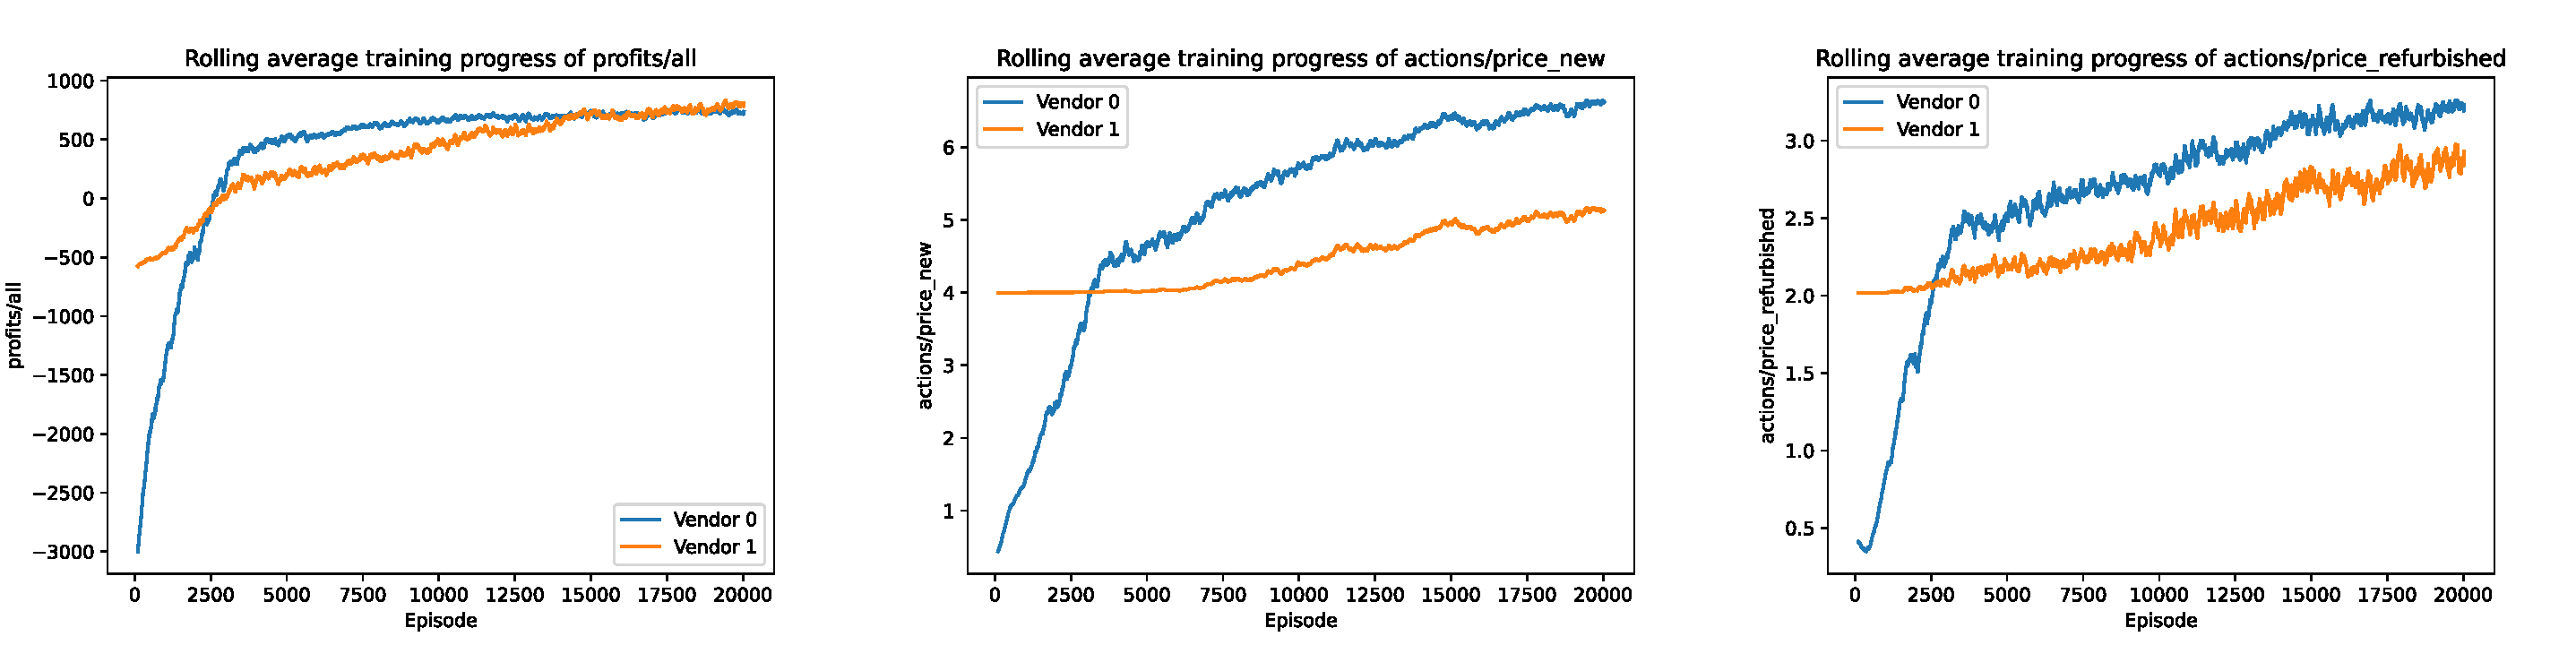
\includegraphics[width=\textwidth]{main/ppo_detailed_analysis.pdf}
	\caption{Detaillierte Betrachtung eines PPO-Trainingsdurchlaufes (Variante mit $\varepsilon=0.2$) analog zu Abbildung \ref{graphic:A2CInstability}}
	\label{graphic:PPOStability}
\end{figure}
In Abbildung \ref{graphic:PPOStability} ist ein detaillierter Blick in einen typischen PPO-Trainingsdurchlauf zu sehen.
Dessen durchschnittliche Performance steigt bis zum Ende auf 8160, und weist bei Return und der Aktionsauswahl eine durchweg stabile Entwicklung auf.

Der Unterschied in der Lerngeschwindigkeit und -stabilität zwischen PPO zu A2C überrascht nicht, er existiert \textit{by design}.
Diese Experimente zeigen, dass PPO in seiner Intention, die Trainingsstabilität zu erhöhen, erfolgreich ist.
Diese Erhöhung der Trainingsstabilität findet dadurch statt, dass die Änderung der stochastischen Policy bei den Trainingsschritten begrenzt wird.
Aus dieser Begrenzung der Policyänderung ist die geringere Lerngeschwindigkeit dann eine logische Schlussfolgerung.

So lässt sich auch erklären, warum der Durchlauf mit $\varepsilon=0.3$ schneller trainiert.
Mit größerem $\varepsilon$ wird pro Sample eine größere Policyänderung erlaubt, was zu schnellerem Training führt.
Allerdings steigt damit wieder das Risiko von Instabilität, weshalb die Parametrisierung des PPO-Algorithmus einen Trade-off zwischen Trainingsgeschwindigkeit und Stabilität eröffnet.
Die Wahl des Standardparameters $0.2$ mag in diesen Experimenten konservativ erscheinen, $0.3$ ist ebenfalls noch recht stabil, weist aber bereits kleinere Abstürze auf.
Das Experiment \ref{graphic:PPODifferentClipping} im Anhang zeigt, wie sich PPO bei größerem $\varepsilon$ verhält.
Es bestätigt $0.3$ als eine gute Wahl.

Eine Beobachtung in Abbildung \ref{graphic:PPOStability} verdient noch einmal besondere Beachtung, weil sie zunächst paradox erscheint:
Obwohl der RL-Agent den regelbasierten Agenten nach etwas Training übertrifft, wird er später wieder wieder überholt.
Das erweckt den Eindruck, als ob der Agent im Verlaufe des Training schlechter würde.
Jedoch ist das Gegenteil der Fall.
Der PPO-Agent erlernt zunächst, die Preise für Neu- und Gebrauchtware höher zu setzen.
Dieses Training dauert aus inzwischen diskutierten Gründen relativ lange, aber bei Neuverkaufspreisen, die größer als vier sind, macht er die Erfahrung, dass der regelbasierte Wettbewerber ihn immer um 1 unterbietet.
Durch wechselseitiges Unterbieten führt eine Preisabwärtsspirale dazu, dass sich der Preis nur knapp überhalb des Einkaufspreises einpegelt.
Die dabei äußerst niedrige Rendite ermöglicht jedoch nur niedrige Gewinne, sodass der Agent in seinem weiteren Training die Erfahrung macht, dass er seinen Gewinn steigern kann, indem er seine Preise höher setzt.
Er wird dann zwar immer noch unterboten, allerdings nur um den Wert eins.
Dabei nimmt er in Kauf, dass mehr Kunden wegen des niedrigen Preises beim Konkurrenten kaufen und dieser bei steigenden Preisen auch an jedem Kunden noch mehr verdient.
Mit den Kunden, die der RL-Agent aber noch bekommt, kann er seine Gewinne im Vergleich zum niedrigpreisigen Markt dennoch steigern.
Der Effekt besteht also darin, dass der RL-Agent in Reaktion auf den ihn immer unterbietenden Konkurrenten diesem einen überproportionalen Gewinnanstieg erlaubt, um selbst mehr Gewinne machen zu können.
Dass sich dieser Effekt so wiederfindet, ist der Tatsache geschuldet, dass das einzige Optimierungskriterium für die Agenten der eigene Gewinn ist.
Eine Rewardformulierung, die ein Übertreffen des Konkurrenten mit einbezieht, wird in Abschnitt \ref{section:mixed_reward_function} behandelt.

\section{Soft Actor Critic}
\label{section:main_sac}
Das in Abschnitt \ref{section:sac} erläuternte Soft-Actor-Critic-Verfahren ist in erster Linie für stetige Aktionsräume entwickelt worden und wird hier auch in der stetigen Variante genutzt.
Bei den hier gezeigten Ergebnissen wurde der Entropiekoeffizient $\alpha$ automatisch trainiert.
Er hat sich bei allen Trainingsdurchläufen bei etwa $1.5$ eingependelt.
Die Grafik ? im Anhang zeigt, dass unterschiedliche manuell eingestellte Entropiekoeffizienten ähnliche Trainingsergebnisse erreichen, wobei sich die Vermutung bestätigt, dass sehr niedrige Entropiekoeffizienten zu wenig Exploration bezwecken und Läufe mit deutlich höheren Entropiekoeffizienten bei schlechterer Leistung verharren.

\begin{figure}[htbp]
	\centering
	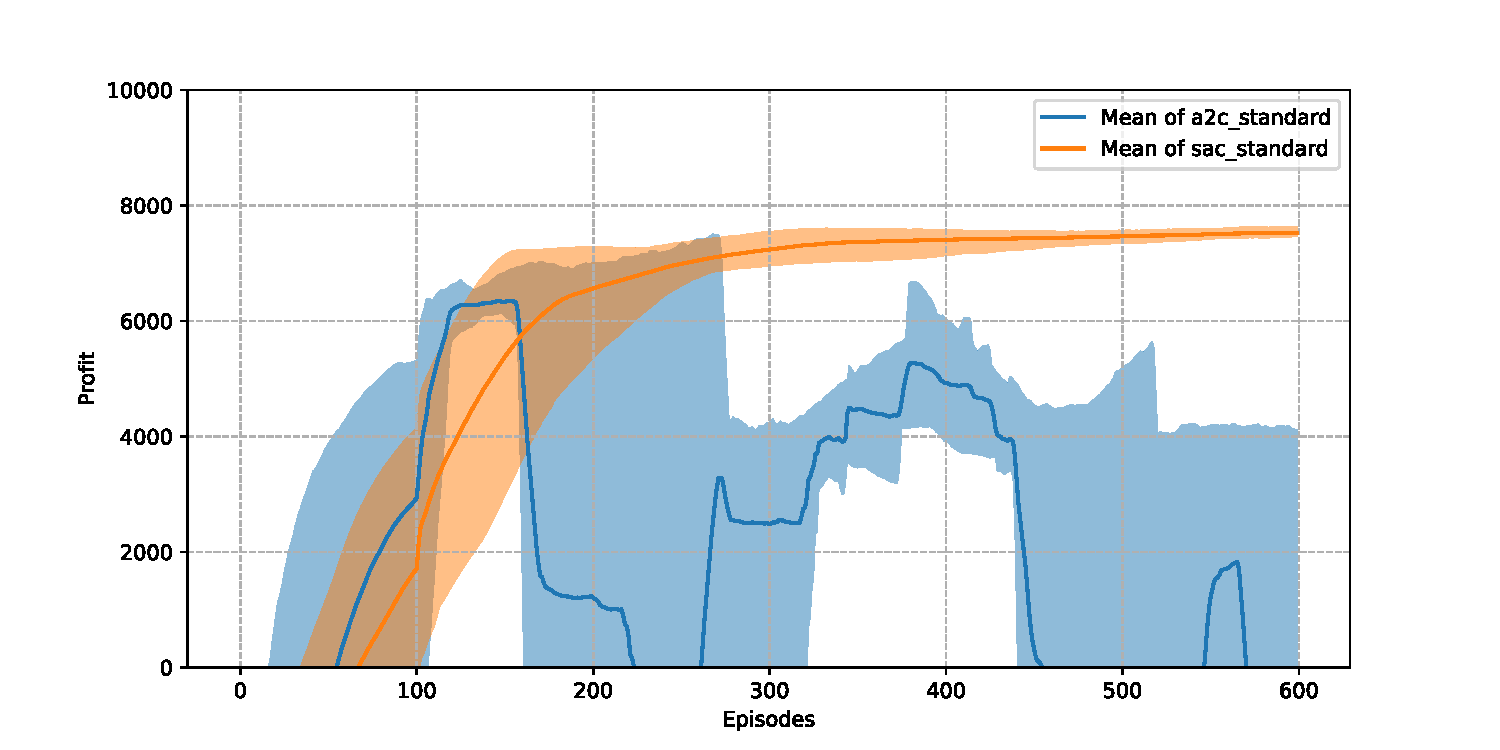
\includegraphics[width=\textwidth]{main/a2c_vs_sac.pdf}
	\caption{Lernkurve von Soft Actor Critic über 600 Episoden, A2C als Vergleich angegeben}
	\label{graphic:SACLearningCurve}
\end{figure}

Grafik \ref{graphic:SACLearningCurve} zeigt die Lernkurve von vier Soft-Actor-Critic-Agenten bei einem Trainingsdurchlauf mit 600 Episoden (300000 Schritte).
Zum Vergleich sind vier Trainingsdurchläufe mit A2C angegeben, die den aus Abschnitt \ref{section:main_ppo} bekannten Verlauf aufweisen.
Bei diesem Diagramm fällt ein sprunghafter Anstieg bei 100 Episoden auf.
Das liegt an dem laufenden Durchschnitt, bei dem nach 100 Episoden die sehr schlechten Ergebnisse direkt am Anfang aus der Mittlung herausfallen.
Dieser Effekt tritt auch bei anderen dieser Lernkurven auf und liegt nur am Diagrammtyp.

Soft-Actor-Critic wurde als Off-Policy-Algorithmus neben dem Erreichen von wettbewerbsfähigen Ergebnissen für zwei Hauptziele entwickelt:
Erstens soll es eine sehr hohe Sample Efficiency haben, was bedeutet, dass es beim Training deutlich weniger Schritten benötigt.
Zweitens soll SAC eine sehr hohe Trainingsstabilität haben.
Die Lernkurve bestätigt, dass Soft-Actor-Critic diese zwei Hauptziele erreicht.
Profitabel arbeitet der Agent nach etwa 70 Episoden, was nur leicht hinter A2C liegt und erheblich besser als PPO ist.
Spitzenperformance wird ähnlich wie bei A2C nach 250 bis 300 Episoden erreicht.
Der weitere Trainingsverlauf ist sehr stabil.
Alle vier Agenten bewegen sich für den Rest des Trainings in einem sehr schmalen Bereich, wobei der Durchschnittsreturn der Agenten bei etwa 7500 konstant bleibt.
Eine Verbesserung der Leistung findet nach etwa 350 Episoden nicht mehr statt.
Der Durchschnitt der acht SAC-Agenten liegt zwar dauerhaft über dem Durchschnitt der A2C-Agenten, aber gute A2C-Durchläufe erreichen bessere Spitzenperformance als die SAC-Agenten.
Die Spitzenergebnisse dieser vier SAC-Durchläufe liegen bei 7550, 7730, 7620 und 7800.
Damit bleiben sie ebenfalls signifikant hinter denen der PPO-Agenten zurück, die zuverlässig über 8000 als Return erzielen.

\begin{figure}[htbp]
	\centering
	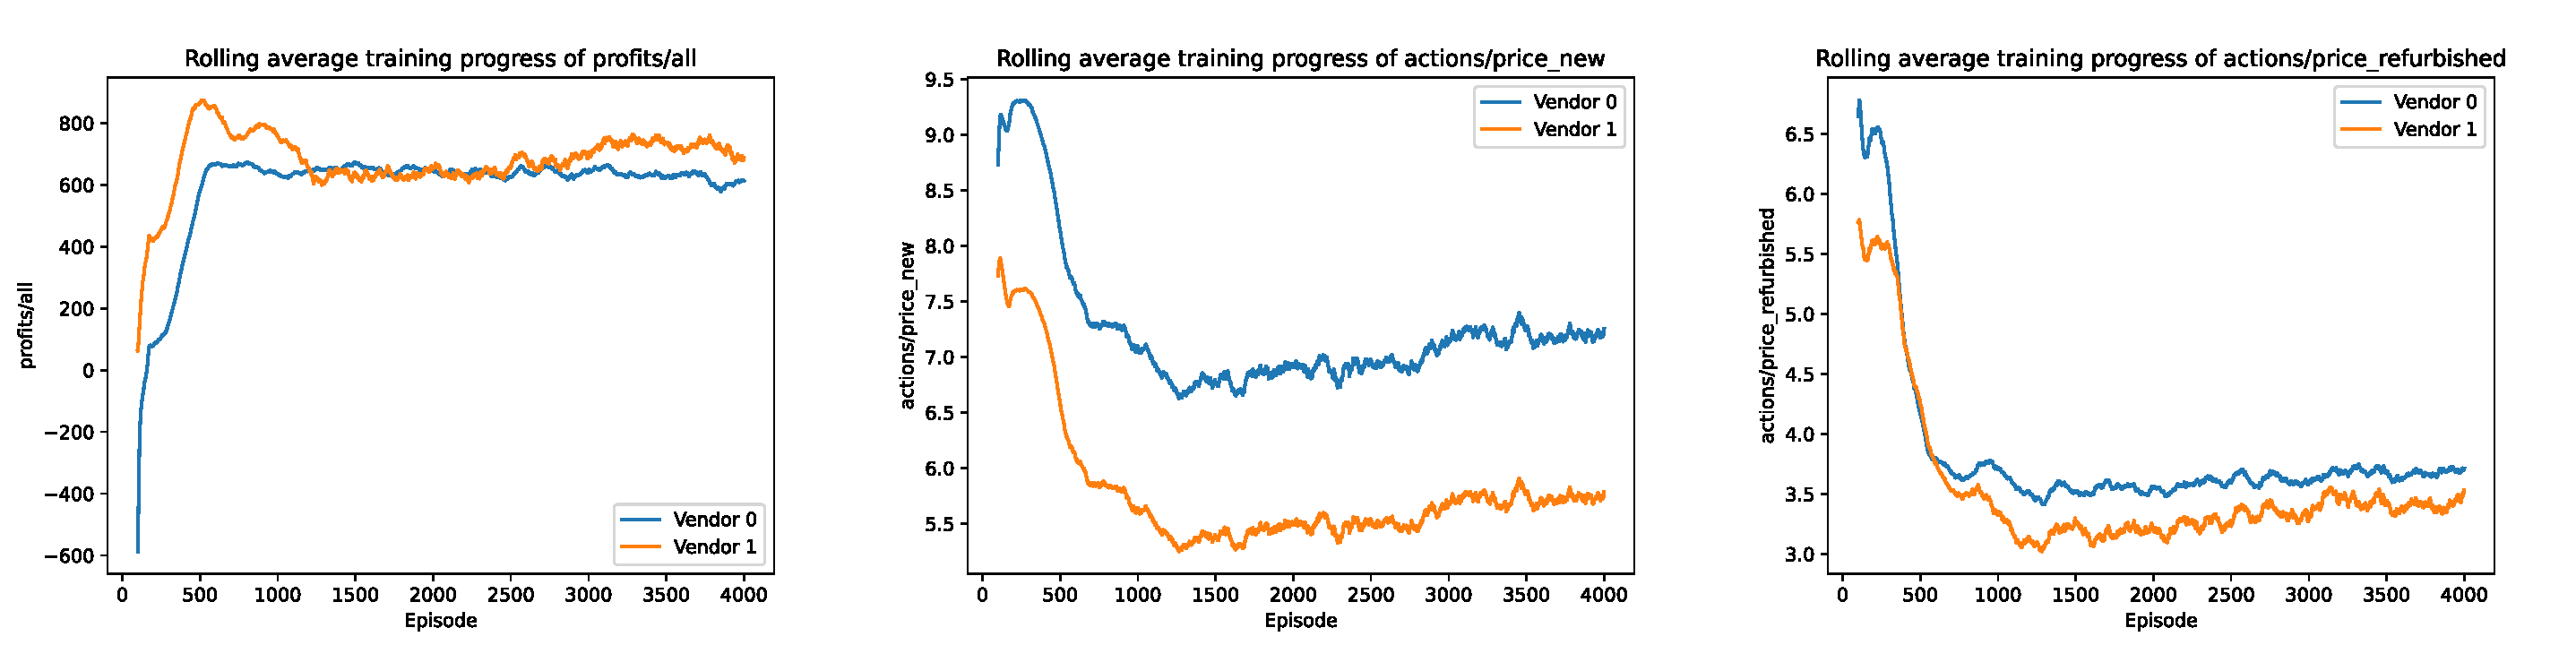
\includegraphics[width=\textwidth]{main/sac_detailed_analysis.pdf}
	\caption{Detaillierte Betrachtung eines SAC-Trainingsdurchlaufes}
	\label{graphic:SACDetails}
\end{figure}

Wie auch für die anderen Algorithmen wurde für SAC ein typischer Durchlauf und die gemittelten Aktionen in Abbildung \ref{graphic:SACDetails} abgedruckt.
Dieser ist stabil und weist abgesehen vom Start mit höheren Werten einen nicht unähnlichen Verlauf im Vergleich zum PPO-Durchlauf auf:
Zunächst sinken die Neupreise, steigen dann leicht an und enden bei 6,4 und 5,4, genau wie bei PPO.

Für die Frage >>Wie lange dauert das Training?<< gibt es zwei mögliche Kenngrößen.
Einmal kann die Anzahl der benötigten Samples bewertet werden, die Sample Efficiency, oder es kann die tatsächliche Zeit auf der Uhr harangezogen werden.
Letztere hängt stark von der Hardware sowie der Geschwindigkeit der Simulation im Vergleich zum Optimieren der Parameter ab.
Bei der für diese Experimente verwendeten Implementierung und Hardware benötigt das Training pro Schritt mit SAC etwa $3.7$ Mal so lang wie mit PPO.
Das Sammeln der Beispiele aus dem Markt nimmt bei PPO etwa 25\% der Trainingszeit ein, bei SAC nur etwa 6\%.
Die Geschwindigkeit des Trainings ist bei A2C und PPO sehr ähnlich.
Rechnet man somit die tatsächliche Trainingszeit, relativiert sich der höhere Samplebedarf bei PPO.
Insbesondere wird deutlich, dass A2C in reinem Zeitbedarf den anderen Algorithmen erheblich überlegen ist.

\section{Den Konkurrenten übertreffen -- eine angepasste Rewardfunktion}
\label{section:mixed_reward_function}
In den bisher untersuchten Lernkurven erreichen die Agenten zwar sehr gute Profite, lassen sich aber vom regelbasierten Konkurrenten übertreffen.
In Abschnitt \ref{section:main_ppo} wurde bereits erklärt, dass dies nicht als Schwäche der Algorithmen zu deuten ist, sondern auf die Rewardfunktion zurückgeführt werden kann, die nur eigenen Profit bewertet.
Nun ist die Maximierung des eigenen Profits keine ungeeignete Kenngröße, dennoch werden Unternehmen ungern ihren Konkurrenten in einem symmetrischen Markt mehr Gewinn überlassen als sich selbst.
Deshalb liegt es nahe, in der Belohnungsfunktion nicht nur die eigenen Profite zu bewerten, sondern auch, ob der Konkurrent übertroffen wird.

Eine Möglichkeit besteht darin, den Markt als \textit{Zero-Sum-Spiel} zu formulieren, indem die Belohnung genau die Differenz aus eigenem Gewinn und dem des Konkurrenten ist.
Diese Formulierung legt den klaren Fokus auf das Übertreffen des Konkurrenten und eröffnet weiterhin möglicherweise das Marktszenario für Erkenntnisse aus der Spieltheorie für Zero-Sum-Spiele.
Allerdings diese Formulierung nicht praxistauglich, weil das Ziel der Profitmaximierung gar nicht bewertet wird.
So kann es passieren, dass bei einer Optimierung auf Differenz zwar der Konkurrent deutlich übertroffen wird, allerdings bei insgesamt niedrigen Gewinnen oder sogar in der Verlustzone.

Deshalb wurde für die folgende Versuchsreihe eine gemischte Rewardfunktion verwendet.
Sie berechnet einfach die Summe aus Profit und Differenz zum Konkurrenten.
Für diese Experimente wurden beide Summanden gleich gewichtet, es könnte aber noch ein Hyperparameter eingefügt werden, um die beiden Ziele Profitmaximierung und Übertreffen des Konkurrenten zu balancieren.

\begin{figure}[htbp]
	\centering
	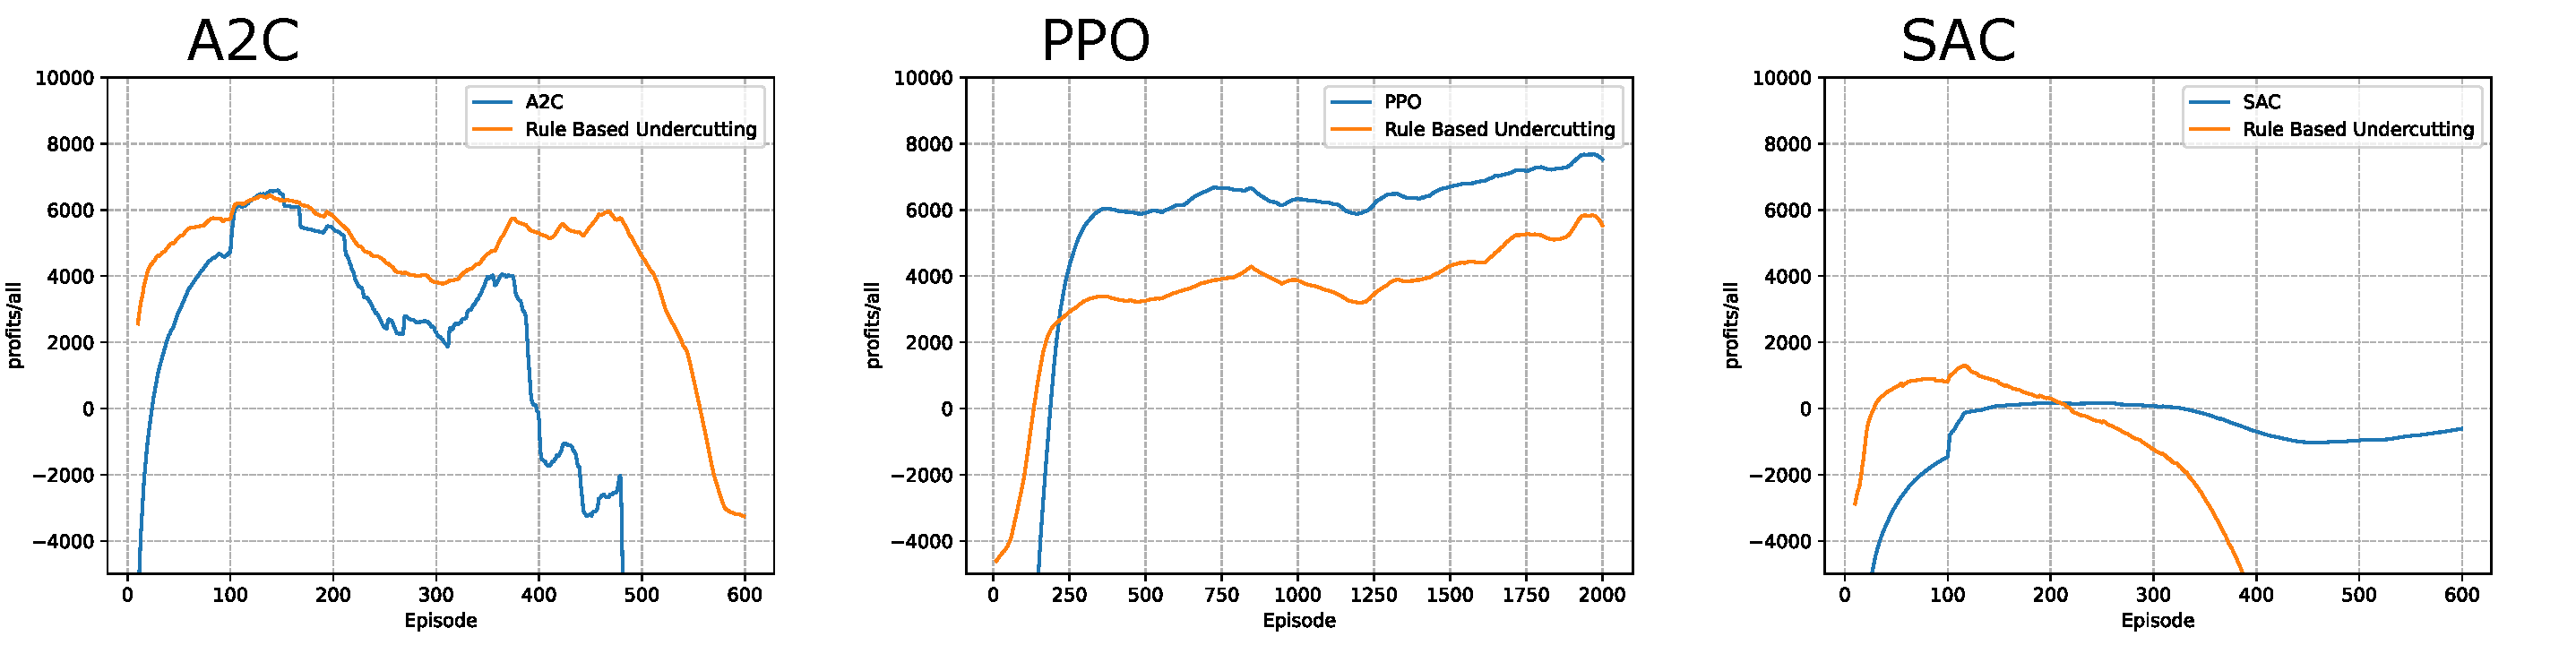
\includegraphics[width=\textwidth]{main/lineplot_mixed_rewards.pdf}
	\caption{Repräsentative Durchläufe der Algorithmen bei gemischter Rewardfunktion}
	\label{graphic:LineplotMixedRewards}
\end{figure}

Im Anhang sind die Lernkurven der Algorithmen mit gemischter Rewardfunktion im vergleich zur Standardrewardfunktion abgedruckt (Abbildungen \ref{graphic:MixedRewardsA2C}, \ref{graphic:MixedRewardsPPO} und \ref{graphic:MixedRewardsSAC}).
Wie erwartet liegen die Gewinne der Agenten niedriger als bei der anderen Rewardfunktion (schließlich sind Gewinne nicht mehr das alleinige Optimierungskriterium), allerdings fällt dieser Unterschied bei den Algorithmen unterschiedlich aus.
Insbesondere erhöht sich durch den Wechsel der Rewardfunktion die Instabilität bei allen Algorithmen.
Ob das Ziel, neben guten Gewinnen die Konkurrenz zu überholen, erreicht wird, zeigt Abbildung \ref{graphic:LineplotMixedRewards}.
Obwohl der A2C-Durchlauf wieder Probleme mit Instabilität zeigt, erreicht er ein durchschnittliches Maximum von 7900, der Konkurrent nur 7200.
Er überholt also bei der veränderten Rewardfunktion den regelbasierten Konkurrenten, und erhält gleichzeitig gute Gewinne.
Beim PPO-Durchlauf ist genau das zu sehen, was Ziel der Anpassung der Rewardfunktion war:
Der PPO-Agent bleibt nach dem ersten Übertreffen des Konkurrenten diesem über das gesamte Training hinweg voraus und erreicht ein Maximum von 8000 im Vergleich zu 6100 des regelbasierten Konkurrenten.
Der Soft-Actor-Critic-Durchlauf erreicht nach der gemischten Rewardfunktion sogar die besten Ergebnisse, obwohl der Agent selbst in die Verlustzone rutscht.
Er hat eine Policy gefunden, bei der der regelbasierte Konkurrent ständig Strafen zahlen muss, weil er keine gebrauchten Produkte liefern kann.
Die Details zu diesem Durchlauf sind interessant und in Abbildung \ref{graphic:ExplanationUnnormalSAC} im Anhang erläutert.
Aus Sicht der Algorithmenanalyse ist es ein bemerkenswertes Resultat, dass der SAC-Agent dazu fähig war, eine solche Strategie zu explorieren und zu entwickeln.
Für die praktische Verwendung ist diese Policy allerdings nicht geeignet.
Der Profit des Agenten sollte beim Design der Rewardfunktion höher gewichtet werden.

\section{Training gegen die eigene Policy}
Die in den Abschnitten \ref{section:main_ddpg}, \ref{section:main_ppo} und \ref{section:main_sac} betrachteten Durchläufe trainierten die RL-Agenten alle gegen den in Abschnitt \ref{section:rulebased} definierten regelbasierten Wettbewerber.
Das erfüllt die theoretischen Anforderungen eines Markov-Entscheidungsprozesses, stellt jedoch für praktische Anwendungen eine Reihe von Problemen auf.
Erstens muss dafür die Policy des Konkurrenten bekannt sein.
Weil jedoch davon ausgegangen werden kann, dass der Konkurrent seine Preisstrategie nicht verraten wird, müsste sie unter Inkaufnahme von Ungenauigkeiten aus historischen Daten geschätzt werden.
Zweitens ist die mittels RL trainierte Strategie nur gegen diese bestimmte regelbasierte Strategie gerichtet.
Ändert der Wettbewerber seine Preisstrategie plötzlich, schwächt das die Performance der RL-Strategie und macht neues Training erforderlich.

Deshalb wünscht man sich eine Strategie, die gegen möglichst viele Wettbewerberstrategien bestehen kann, und nicht auf eine spezielle overfittet ist.
Deepmind hatte eine ähnliche Herausforderung beim Training von Go- und Schachstrategien, das durch Self-Play gelöst wurde. \cite{Silver2017, https://doi.org/10.48550/arxiv.1712.01815}
Für diesen Markt wurde eine Self-Play Variante entwickelt, bei der ein RL-Agent weiterhin auf einem Duopol-Markt trainiert, aber die Policy des Wettbewerbers die eigene Policy ist.
In der programmiertechnischen Umsetzung wird dann für den Gegner ein Zeiger auf den RL-Agenten übergeben, der schließlich auch die Policyfunktion implementiert.
Dadurch, dass der Agent stets gegen sich selbst spielt, wird die Markov-Eigenschaft verletzt, dennoch zeigen die Ergebnisse Trainingserfolg.
Die Motivation hinter Self-Play ist, dass der Agent einerseits stets einem ebenbürtigen Gegner gegenübersteht, aber andererseits auch, dass er ständig Strategien gegen die eigene entwickelt, die dann wiederum herausgefordert werden.
Dadurch soll der Agent gegen eine Vielzahl von Policies gestählert werden.
Experimente mit Self-Play wurden mit den Algorithmen durchgeführt, die sich in der vorangegangenen Analyse als grundsätzlich geeignet für diesen Markt erwiesen haben: A2C, PPO und SAC.
Dabei wurde die gesamte Versuchsreihe mit der normalen Rewardfunktion und der gemischten Rewardfunktion aus Abschnitt \ref{section:mixed_reward_function} durchgeführt.

\begin{figure}[htbp]
	\centering
	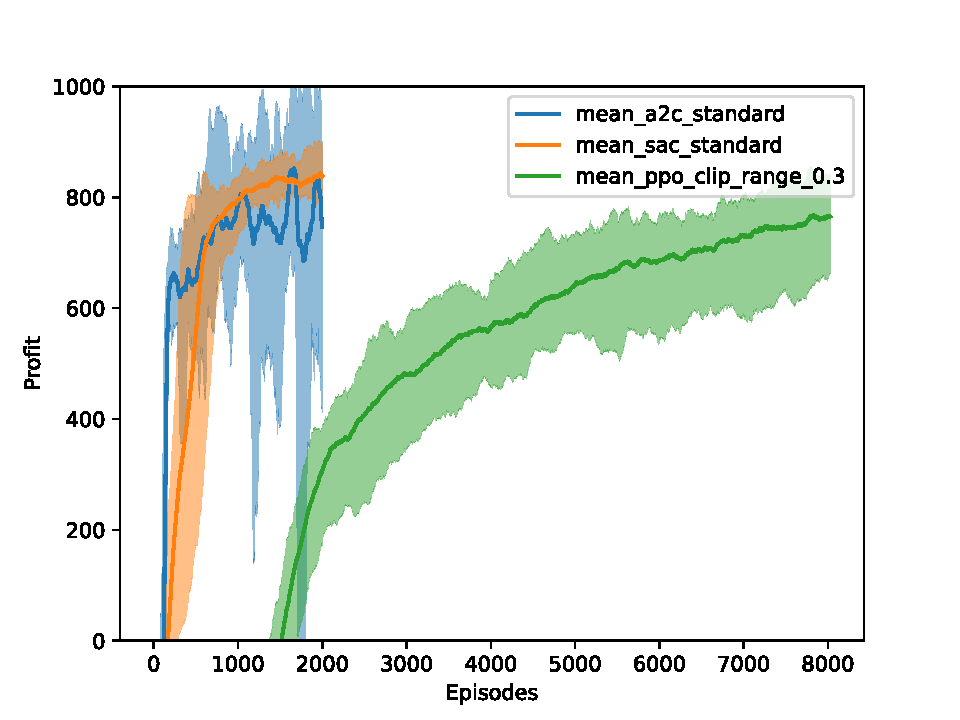
\includegraphics[width=\textwidth]{main/self_play.pdf}
	\caption{Lernkurve von A2C, PPO und SAC beim Self-Play; die Algorithmen wurden über 2000 Episoden trainiert}
	\label{graphic:SelfPlayLearningCurve}
\end{figure}
In der Abbildung \ref{graphic:SelfPlayLearningCurve} sind die Lernkurven der drei Algorithmen beim Training gegen sich selbst abgedruckt.
Die Lernkurven bei gemischter Rewardfunktion sehen ähnlich aus und sind im Anhang in Abbildung \ref{graphic:SelfPlayMixedLearningCurve} abgedruckt.
Diese Kurven zeigen zunächst, dass Lernerfolg bei allen dieser drei Agenten erreicht wird.
Sie alleine können allerdings nicht aussagen, ob die Agenten sich tatsächlich gegen die Konkurrenz behaupten können.
Deshalb dürfen auch die Returns dieser Lernkurven nicht mit den aus den vorigen Abschnitten verglichen werden.

\begin{figure}[htbp]
	\centering
	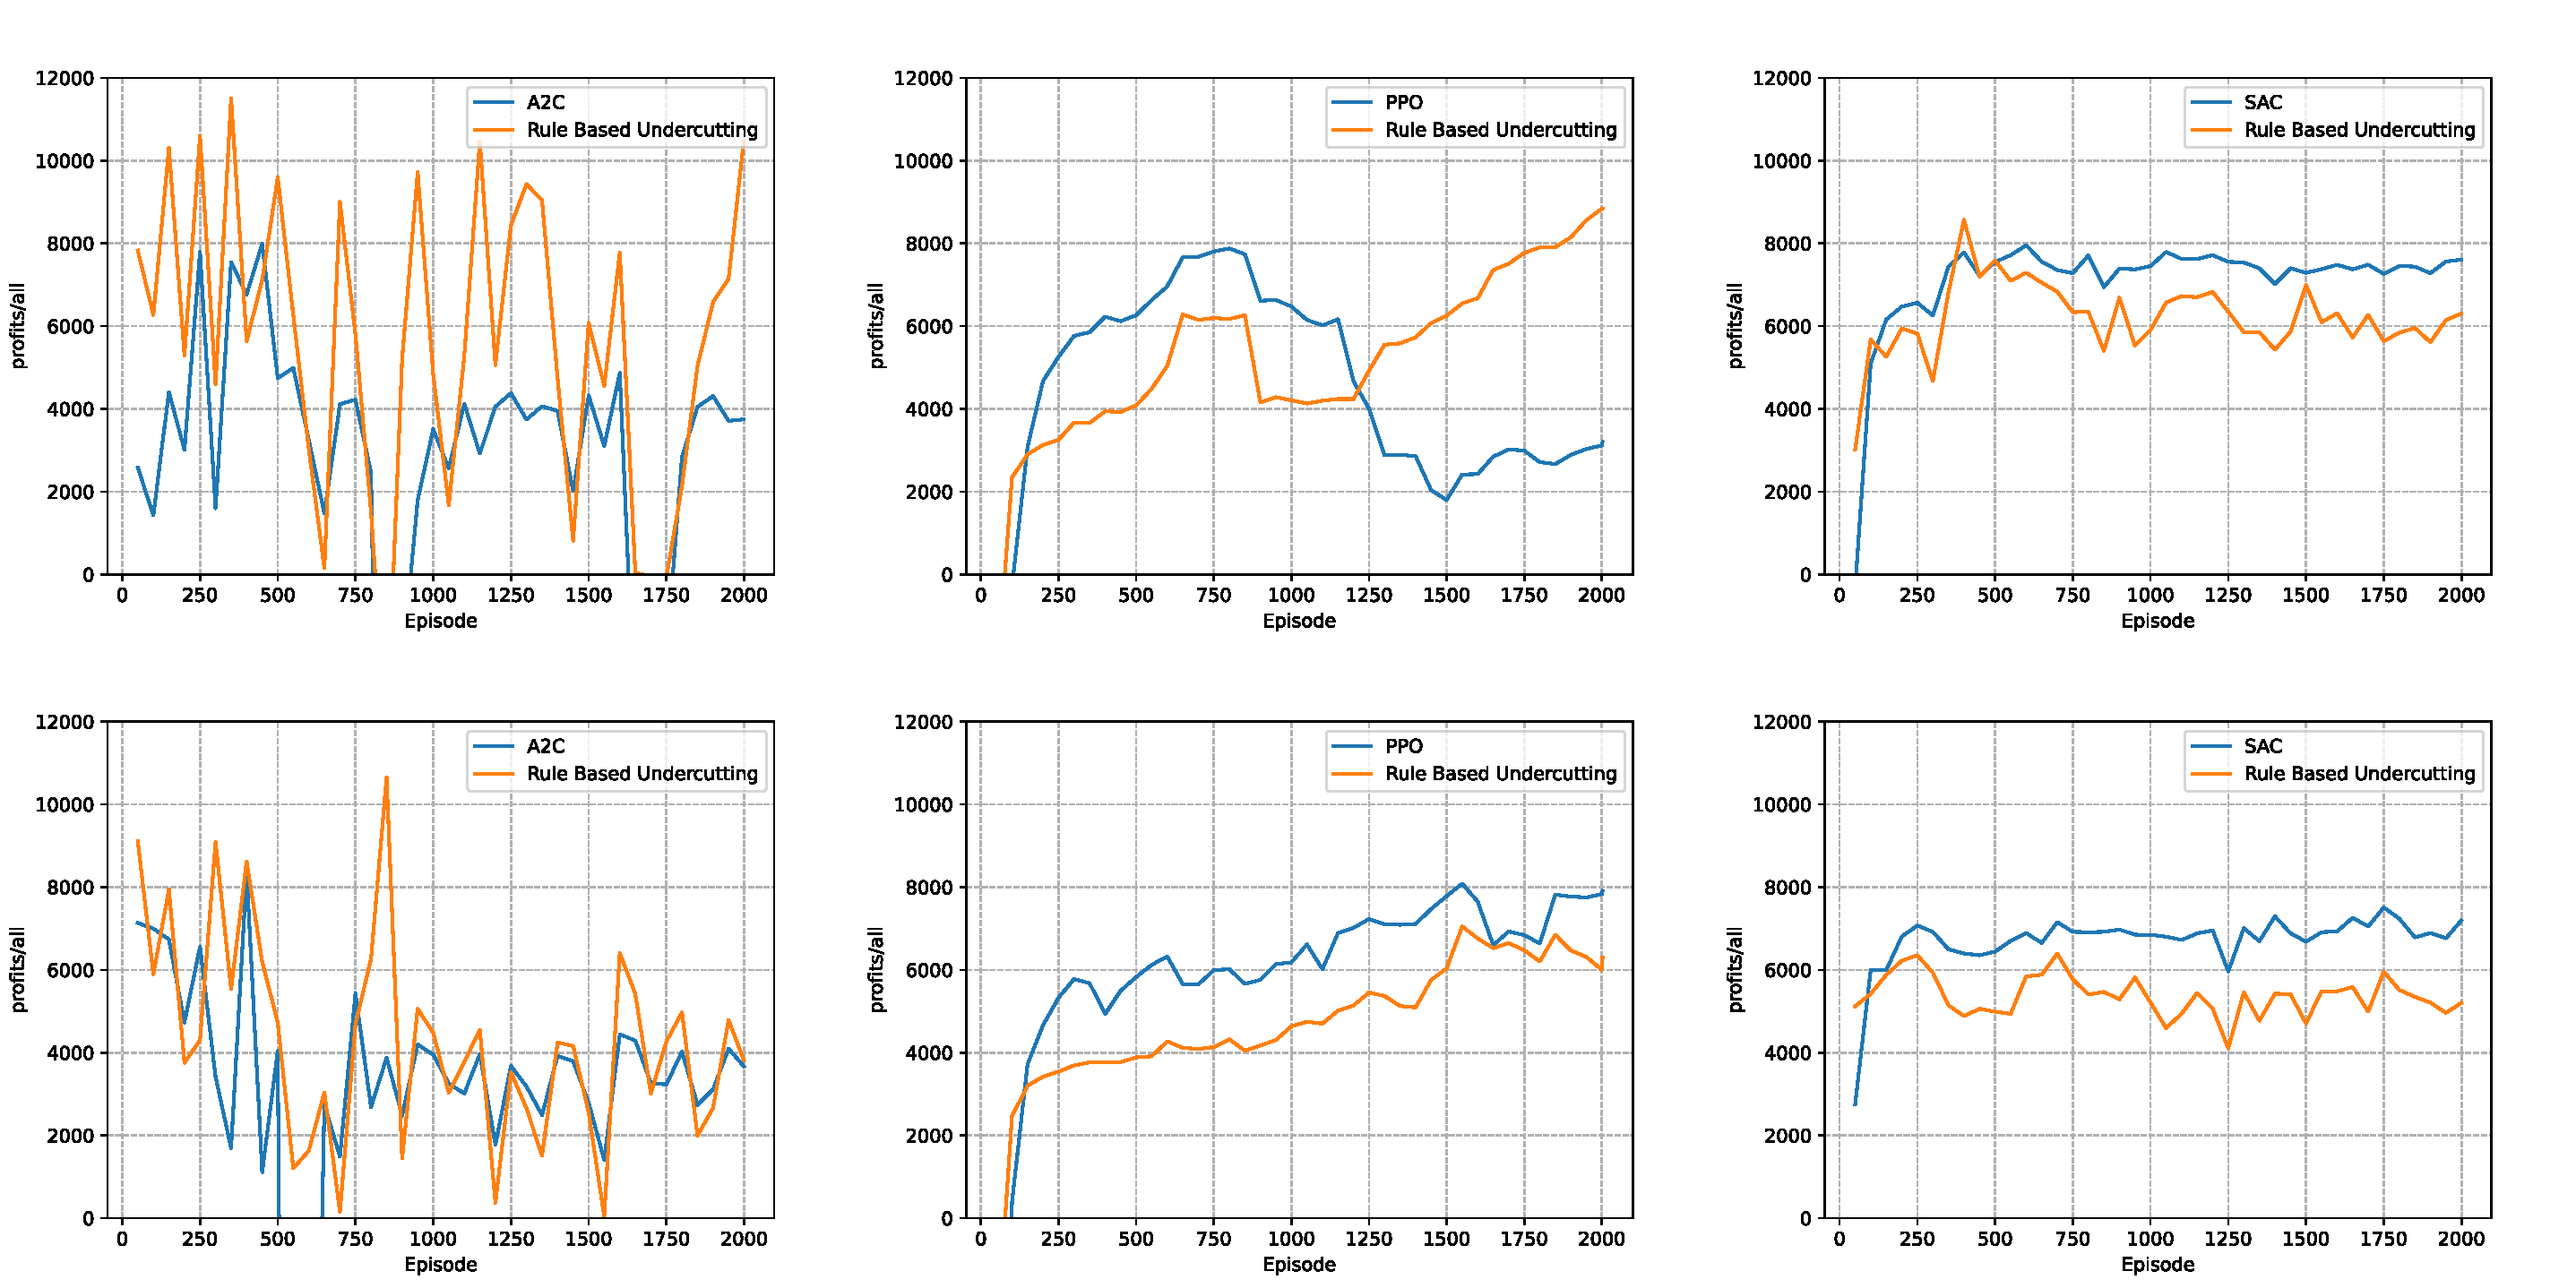
\includegraphics[width=\textwidth]{main/self_play_detailed.pdf}
	\caption{Repräsentative Self-Play Durchläufe; Spaltenweise nach Agenten: (links) A2c, (mittig) PPO, (rechts) SAC; obere Zeile mit normaler Rewardfunktion, untere Zeile mit gemischter Rewardfunktion}
	\label{graphic:SelfPlayDetails}
\end{figure}
Um Vergleichbarkeit herstellen zu können, wurde während des Self-Plays alle 50 Episoden ein Modell gespeichert und jedes dieser Modelle anschließend für 25 Episoden getestet.
Damit wurden akkurate Lernkurven erstellt, die das beim Self-Play trainierte Modell mit dem regelbasierten Agenten vergleichen.
Für die drei Algorithmen und die zwei Rewardfunktionen wurde ein mittlerer Durchlauf ausgewählt und in der Abbildung \ref{graphic:SelfPlayDetails} veranschaulicht.
Bei beiden Rewardfunktionen haben die Agenten den Markt erfolgreich erlernt und können sich auch in dem Benchmark gegen den regelbasierten Konkurrenten behaupten.
So liegen die Spitzenwerte aller Agenten im Benchmark bei 8000 oder knapp darunter, allerdings mit starken Schwankungen bei A2C.
Von den A2C-Agenten erreichten einige kein Niveau von 5000.
Die Auswirkungen der gemischten Rewardfunktion sind gerade bei A2C und SAC deutlich.
Dass während des Trainings die Differenz zwischen eigenem und gegnerischen Profit mit als Optimierungskriterium verfolgt wird, führt tatsächlich dazu, dass der durch Self-Play trainierte Agent auch im Vergleich mit dem regelbasierten Konkurrenten sich zumindest nicht übertreffen lässt (A2C) oder den Konkurrenten im Gegensatz zur normalen Rewardfunktion abhängt (SAC).
Obwohl die Benchmarkergebnisse erwartungsgemäß nicht ganz an die Ergebnisse des Trainings direkt gegen den regelbasierten Agenten heranreichen, so sind sie nahe daran.
Das ist bemerkenswert, da diese Erfolge im Benchmark erreicht wurden, ohne den regelbasierten Wettbewerber je vorher gesehen zu haben.
Damit können diese Ergebnisse als erfolgreich gewertet werden.
Die Fähigkeiten vom Training gegen die eigene Policy werden in diesem Setup bestätigt.

\section{Partielle Beobachtungen}
Für die Markov-Eigenschaft ist ein sechsdimensionaler Aktionsraum erforderlich.
Jedoch ist die Beobachtung mancher der verwendeten Größen in der Praxis nicht machbar.
So wird der Konkurrent sich nicht ins Lager schauen lassen, und die Anzahl der Produkte in Zirkulation ist schwer zu schätzen.
Deshalb drängt sich die Frage auf, ob die Algorithmen auch ohne diese beiden Informationen funktionieren.

\begin{figure}[htbp]
	\centering
	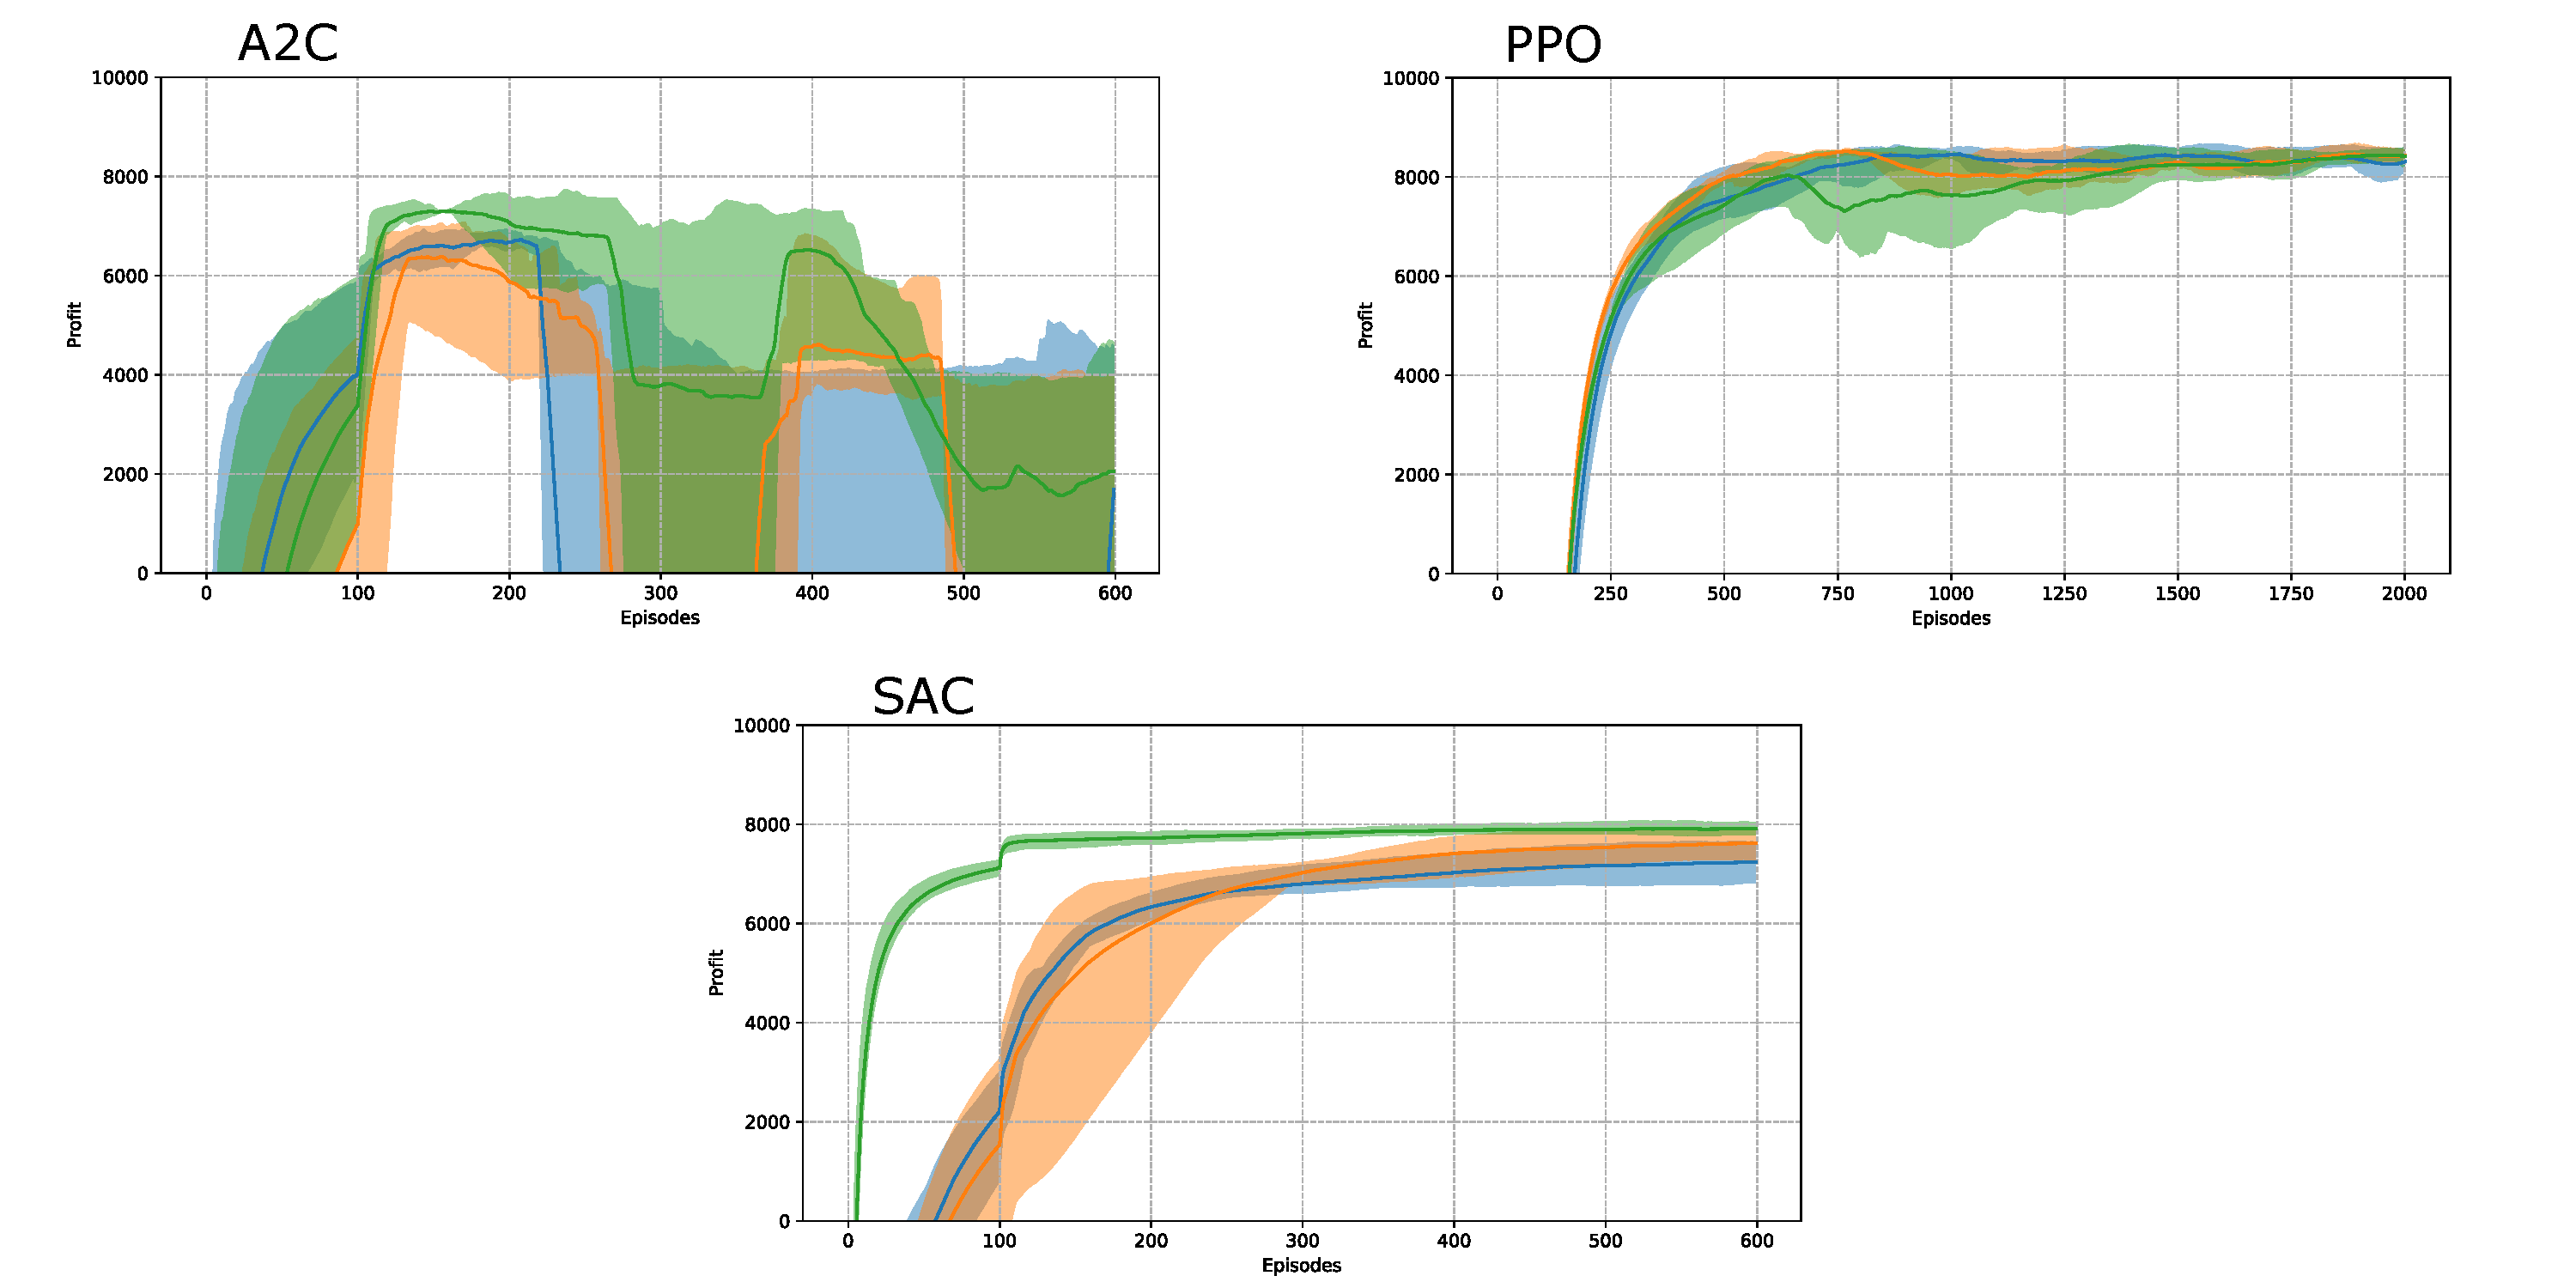
\includegraphics[width=\textwidth]{main/partial_observation.pdf}
	\caption{Lernkurven von A2C, PPO und SAC bei vollständiger im Vergleich zu partieller Beobachtung; (blau) vollständige Beobachtung, (orange) Lagerstand des Konkurrenten wird nicht bereitgestellt, (grün) Lagerstand des Konkurrenten und Anzahl der Produkte in Zirkulation werden nicht bereitgestellt}
	\label{graphic:PartialObservation}
\end{figure}

In Abbildung \ref{graphic:PartialObservation} sind die Lernkurven der drei Algorithmen beim Training gegen die unterbietende, regelbasierte Strategie dargestellt.
Das Ergebnis fällt dabei äußerst überraschend aus.
Die Erwartung, dass weniger Informationen zu schlechteren Ergebnissen führen müssten, erfüllt sich nicht.
Bis auf eine leicht verschlechterte Stabilität ist die Performance bei PPO ähnlich.
Dieses geringfügige Absinken der Stabilität lässt sich vermutlich direkt durch des Fehlens von Informationen erklären.
Bei A2C verbessert sich ohne diese Informationen die Performance, und SAC sogar deutlich.
Während der SAC-Agent, dem nur der Lagerstand des Konkurrenten vorenthalten wird, recht ähnliche, leicht verbesserte Ergebnisse wie der mit vollständiger Information erzielt, ist der, bei bei denen zusätzlich die Information über die Anzahl der Produkte in Zirkulation fehlt, deutlich besser.
Es senkt sich nicht nur die Zeit bis zum Erreichen der Spitzenperformance auf unter 100 Episoden, sondern es verbessert sich sogar die endgültige Performance.
Damit reicht die Leistung näher, aber nicht ganz an die von PPO heran.
Das ist eine wichtige Erkenntnis mit Blick auf die praktische Anwendbarkeit, und dennoch stellt sich die Frage, wie sich die unerwartet gute Leistung mit unvollständiger Information erklären lässt.

Zur Erklärung ist zunächst heranzuführen, dass die ausgelassenen Informationen nur eine nachgeordnete Rolle spielen.
Sie erklären zwar zu einem Teil den künftigen Zug des Konkurrenten und die Anzahl der verkaufswilligen Eigentümer, allerdings sind die Auswirkungen so indirekt, dass sie schwer für die Verbesserung einer Policy zu verwerten sind. \footnote{Die regelbasierten Konkurrenten verwenden diese Information auch nicht}
Ein höherdimensionaler Beobachtungsraum stellt zudem grundsätzlich für die Agenten eine Herausforderung dar.
Es steigt dann der Bedarf an Samples, Muster in den Daten sind schwerer zu erkennen.

\begin{figure}[htbp]
	\centering
	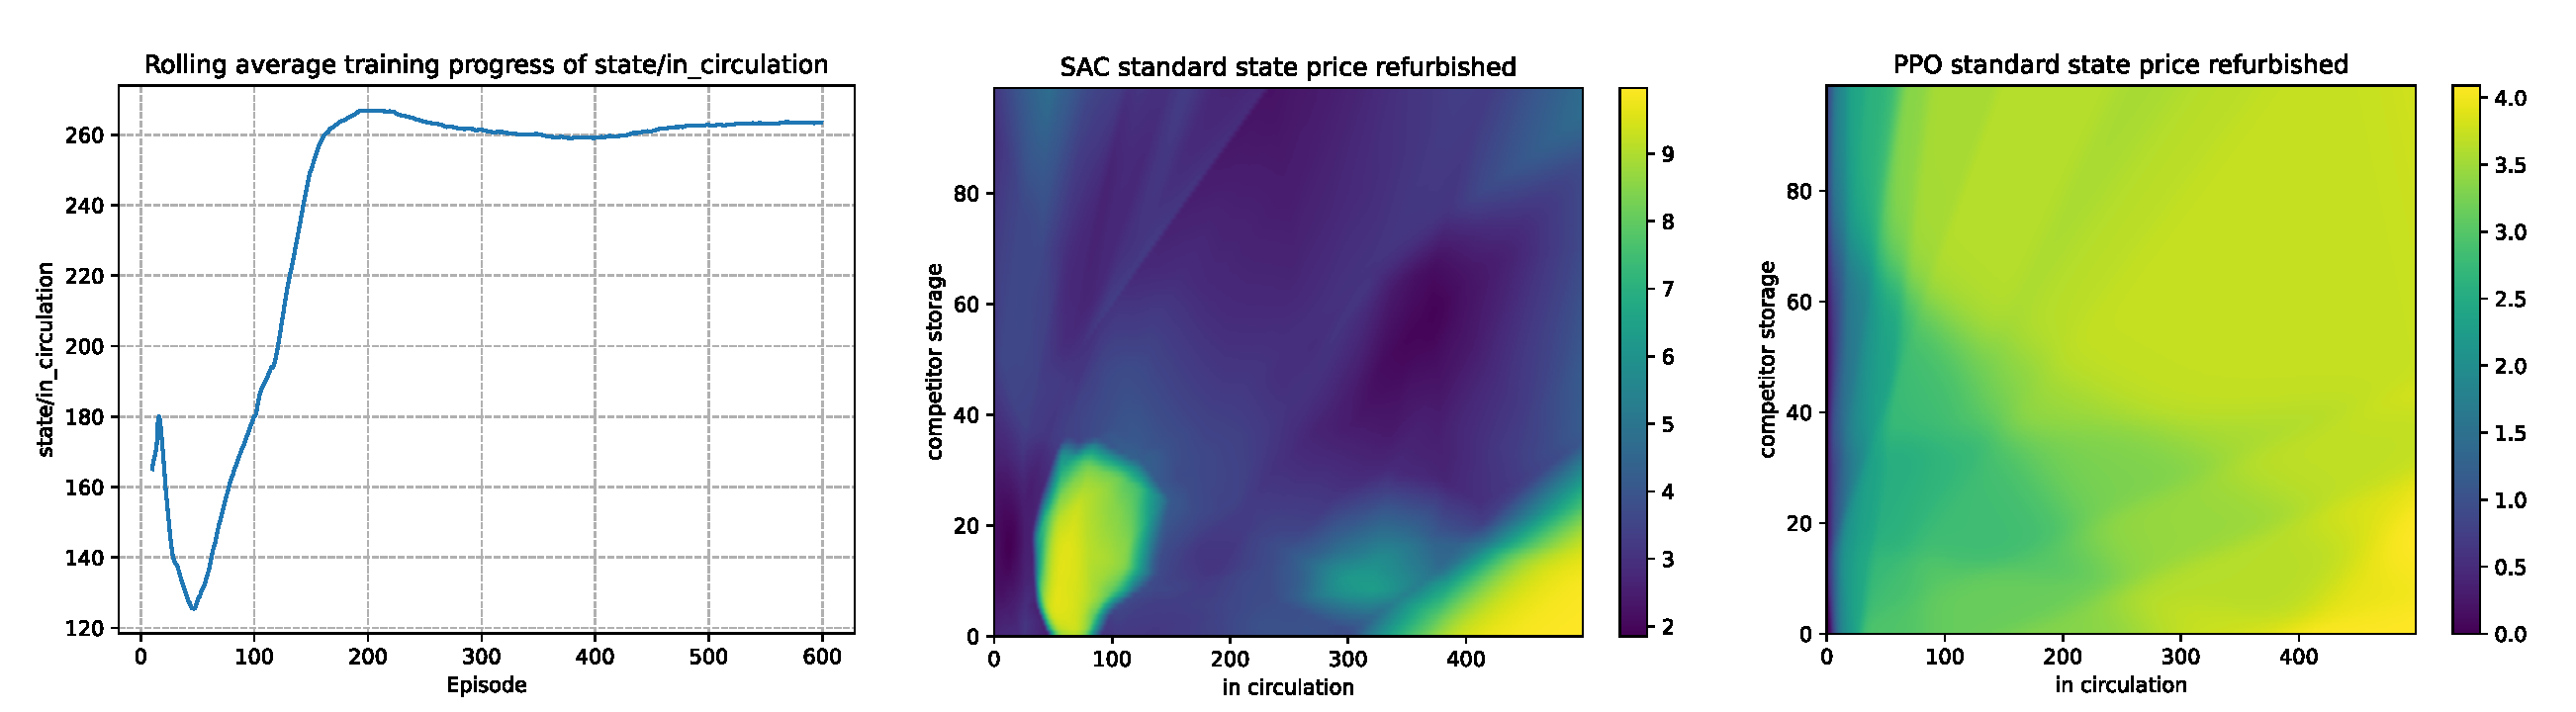
\includegraphics[width=\textwidth]{main/sac_in_circulation_dependend_explanation.pdf}
	\caption{Betrachtung der Agenten mit vollständiger Information: (links) Verlauf des \textit{in-circulation}-Zählers im SAC-Training, (mittig und rechts) Gebrauchtpreis in Abhängigkeit von \textit{in-circulation} und Lagerstand des Konkurrenten bei SAC und PPO; andere Argumente sind dabei fest auf einen Wert gewählt, der typisch bei einem Trainingsdurchlauf ist (eigener Lagerstand: 25, Neupreis Konkurrent: 6, Gebrauchtpreis Konkurrent: 4, Rückkaufpreis Konkurrent: 0)}
	\label{graphic:InCirculationExplain}
\end{figure}
Für das spezielle Phänomen genügt die höhere Dimension bei SAC allerdings nicht.
Ein weiterer Erklärungsansatz drängt sich auf.
Zunächst kann aus Abbildung \ref{graphic:InCirculationExplain} (Mitte) gelesen werden, dass der SAC-Agent Abhängigkeiten der beiden Argumente (Zähler der Anzahl in Zirkulation und Lagerstand des Konkurrenten) erlernt.
Dass sich eine nahezu optimale Policy so verhalten sollte, ist angesichts der geringen Bedeutung der beiden Argumente auszuschließen, was die Policy des deutlich erfolgreicheren PPO-Agenten bestätigt.
Wie man es erwarten würde, hängt sie kaum von diesen beiden Argumenten ab.
Die niedrigere Spitzenperformance von SAC lässt sich vermutlich durch derartige Schwächen der Policy erklären.
Für die von SAC erlernte Policy lässt sich eine Erklärung in der Funktionsweise von Soft Actor Critic finden.
Sie basiert darauf, dass bei weiterentwickelten Policies im Markt mehr Produkte in Zirkulation sind.
Das ist in Abbildung \ref{graphic:InCirculationExplain} (links) gezeigt und liegt daran, dass wenig trainierte Policies im Gegensatz zu den weiterentwickelten oft zu viel zurückkaufen (und dabei zu viel Geld ausgeben).
Das bedeutet, dass gerade am Anfang der Experiencebuffer nur mit Zustandsübergänge mit niedrigen \textit{in-circulation}-Werten gefüllt wird.
Diese Samples bleiben im Experiencebuffer, sind aber für das spätere Training nicht mehr hilfreich und können die Anomalien in der Policy erklären.
So liegt eine starke Anomalie in der Policy im Bereich zwischen 50 und 150 Produkten in Zirkulation, genau der Bereich, aus dem die frühen Samples stammen.
Das Entfallen des \textit{in-circulation}-Eintrages verbessert also die Performance des SAC wohl deshalb, weil dieser dann nicht mehr die Möglichkeit hat, mit missweisenden Samples tatsächlich nicht existente Zusammenhänge zu erlernen.
Es ist damit als Schwäche von SAC gegenüber dem On-Policy-Verfahren PPO zu verzeichnen, dass es weniger gut in der Lage ist, die geringe Relevanz dieses Attributes selbstständig zu erlernen.

\section{Vergleich im Monopol}
In den vorigen Abschnitten wurden die Algorithmen in einem Recommerce-Duopol mit einem regelbasierten, unterbietenden Konkurrenten getestet.
Für reale Anwendungen sind aber viele verschiedene Szenarien möglich.
Es ist daher von Interesse, wie die Algorithmen auf verschiedenen Marktszenarien abschneiden, die in der Praxis auftreten können.
Ein Szenario, das leichter ist sein dürfte, ist das Monopol.
Hier ist der RL-Agent der einzige Anbieter, während weiterhin die gleiche Anzahl von Kunden den Markt besucht.
Die anderen Dynamiken des Marktes sind unverändert.
Als Rewardfunktion wird der Gewinn des Agenten gewählt -- Vergleiche mit Konkurrenten erübrigen sich im Monopol.

\begin{figure}[htbp]
	\centering
	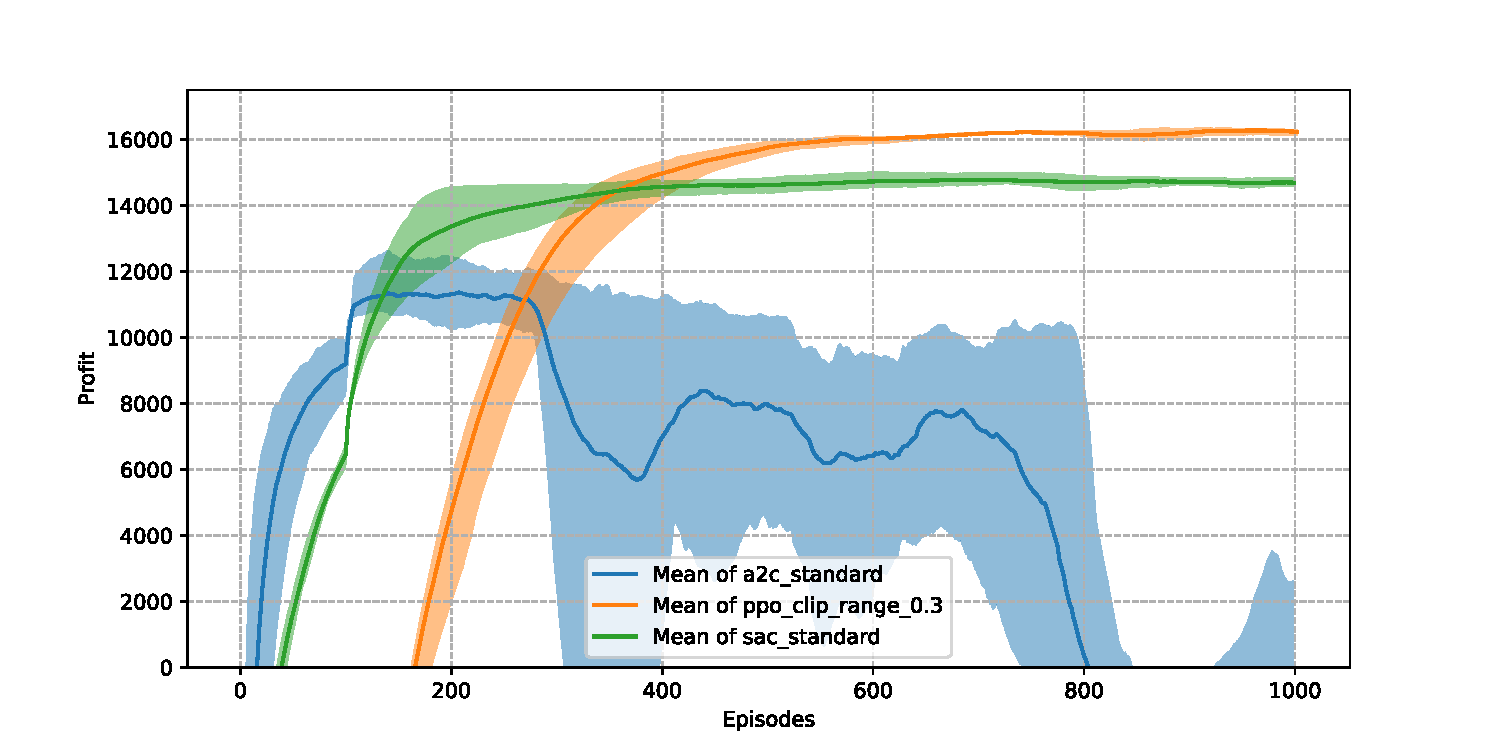
\includegraphics[width=\textwidth]{main/comparison_monopoly.pdf}
	\caption{Lernkurven von A2C, PPO und SAC in einem Monopolszenario über 1000 Episoden}
	\label{graphic:MonopolyComparison}
\end{figure}

Abbildung \ref{graphic:MonopolyComparison} zeigt die Lernkurven der drei Agenten auf dem Monopolmarkt mit vollständiger Information.
Dabei stechen sofort die Parallelen zum Duopol-Markt ins Auge:
\begin{enumerate}
	\item Die relative Reihenfolge der Agenten bei der Lernkurve ist die gleiche: PPO schneidet am besten ab, dann SAC vor A2C.
	\item A2C erreicht als erstes die Gewinnzone, dann folgt SAC und zuletzt PPO.
	\item Das Training von PPO und SAC ist sehr stabil, A2C-Training ist von Abstürzen geprägt.
\end{enumerate}
Auch wenn der Monopol-Markt einfacher ist, so benötigt das Training nicht erheblich weniger Samples.
Vergleicht man den Punkt, an dem die Algorithmen keine deutlich besseren Ergebnisse mehr erreichen, liegt A2C in beiden Setups bei 100 bis 200 Episoden, SAC bei etwa 300 Episoden und PPO bei etwa 600 Episoden.

Im Monopol erzielen diese drei Algorithmen etwa doppelt so hohe Gewinne wie im Duopol.
Auf der einen Seite ist das plausibel, schließlich müssen sie sich den Markt nicht mehr aufteilen.
Auf der anderen Seite könnte man aber erwarten, dass die Gewinne sogar höher ausfallen, indem die Monopolsituation durch Verlangen höherer Preise ausgenutzt wird.
Dass das nicht geschieht, liegt an der begrenzten Kaufbereitschaft der Kunden, gerade bei höheren Preisen.
Im Anhang in Abbildung \ref{graphic:PPOMonopolyDuopoly} wird dazu ein PPO-Durchlauf im Monopol mit dem im Duopol mit Blick auf Verkaufszahlen verglichen.

\section{Vergleich im Oligopol}
Als weiteres Szenario wird das Oligopol untersucht.
Dabei tritt der RL-Agent gegen die folgenden Agenten an:
\begin{enumerate}
	\item eine Verallgemeinerung des bekannten regelbasierten Agenten (unterbietet das Minimum der anderen um eins),
	\item einen regelbasierten Agenten, der mithilfe der Preise zwar sein Lager reguliert, aber nicht auf die anderen Agenten reagiert,
	\item einen Agenten, der feste Preise hat (6 als Neupreis, 3 als Gebrauchtpreis und 2 als Rückkaufpreis) und
	\item einen Agenten, der speziell für das Oligopolszenario erstellt wurde.
	Als Neupreis unterbietet er den Median der anderen Anbieter, und reguliert sein Lager so, dass es etwa 7 Produkte enthält.
\end{enumerate}
Jeder Schritt wird dann in Fünftel zerlegt, die Anbieter setzen ihre Preise reihum.
In jedem dieser Fünftel kommen vier Kunden zum Marktplatz, insgesamt also weiterhin 20.
Das sonstige Verhalten des Marktes bleibt unverändert.
Der Beobachtungsraum ist 18-dimensional (\textit{in-circulation}, eigener Lagerstand und für jeden der vier Konkurrenten drei Preise sowie der Lagerstand).
Damit handelt es sich um das komplexeste Szenario, das behandelt wurde.

\begin{figure}[htbp]
	\centering
	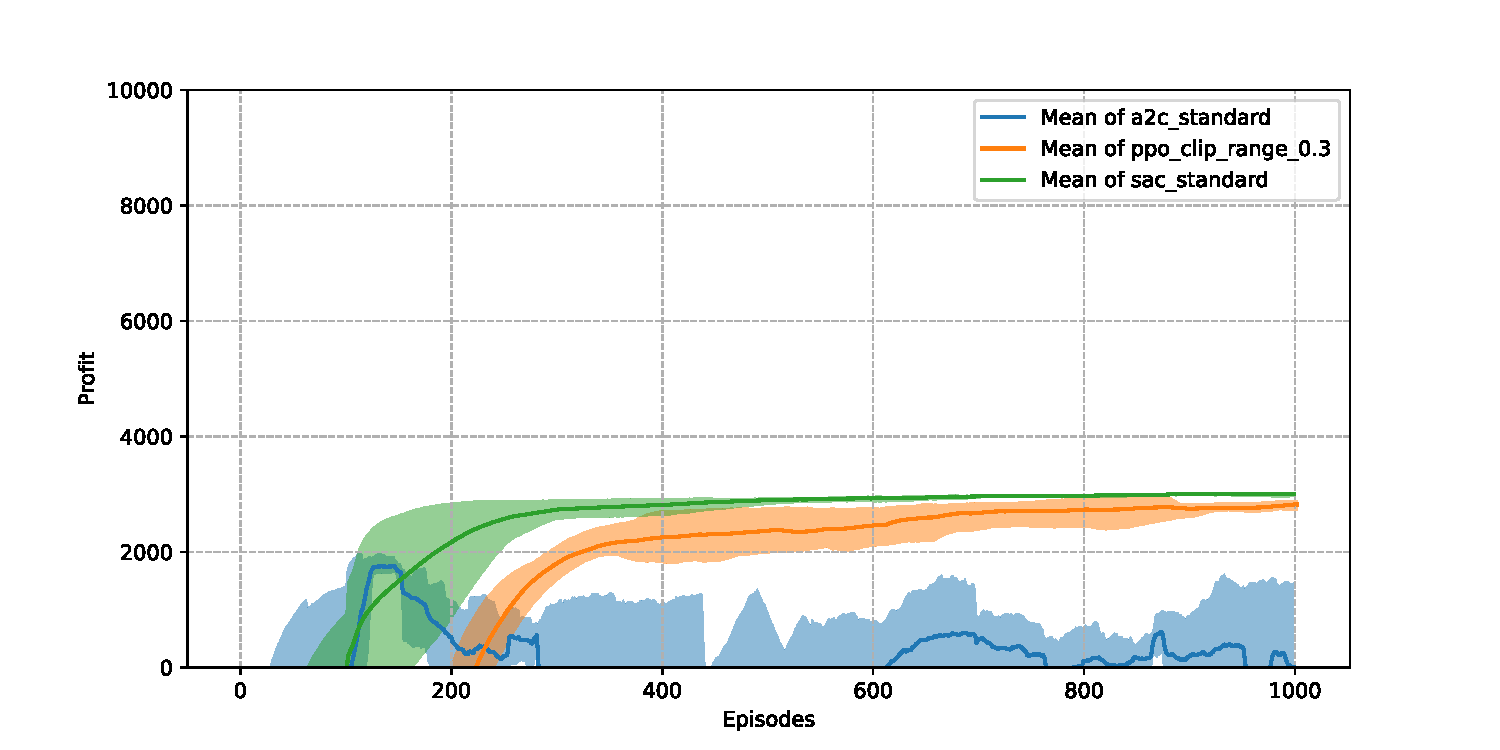
\includegraphics[width=\textwidth]{main/comparison_oligopoly.pdf}
	\caption{Lernkurven von A2C, PPO und SAC in einem Oligopolszenario über 1000 Episoden mit normaler Rewardfunktion und vollständiger Beobachtung}
	\label{graphic:OligopolyComparison}
\end{figure}

Grafik \ref{graphic:OligopolyComparison} zeigt die Lernkurven auf diesem Oligopolszenario.
Die RL-Agenten erreichen auch hier Lernerfolg, wobei die Gewinne selbstverständlich niedriger ausfallen, da sich die gleiche Anzahl von Kunden auf deutlich mehr Anbieter verteilt.
Wie auch in den anderen Experimenten, zeigen PPO und SAC stabile Lernkurven.
Bei A2C zeigen sich die bekannten Instabilitäten, aber die Spitzenperformance bleibt tatsächlich nur leicht hinter der der anderen Algorithmen zurück.
Äußerst interessant ist bei diesem Versuch, dass der SAC-Algorithmus besser abschneidet als PPO, der bei den anderen Experimenten in der Spitzenleistung überlegen war.
Obwohl eine ursächliche Begründung dafür hier nicht geliefert werden kann, so wurde die Leistungsfähigkeit von Soft Actor Critic in hochdimensionalen Benchmarks bereits im Originalpaper hervorgehoben. \cite{haarnoja2018soft}
Das Experiment wurde ebenfalls mit der gemischten Rewardfunktion durchgeführt.
Dessen Ergebnisse sind ähnlich, allerdings finden die SAC-Durchläufe in einer deutlich größeren Spanne statt.
Die Lernkurven dazu sind im Anhang in Abbildung \ref{graphic:OligopolyMixedComparison} abgedruckt.

\begin{figure}[htbp]
	\centering
	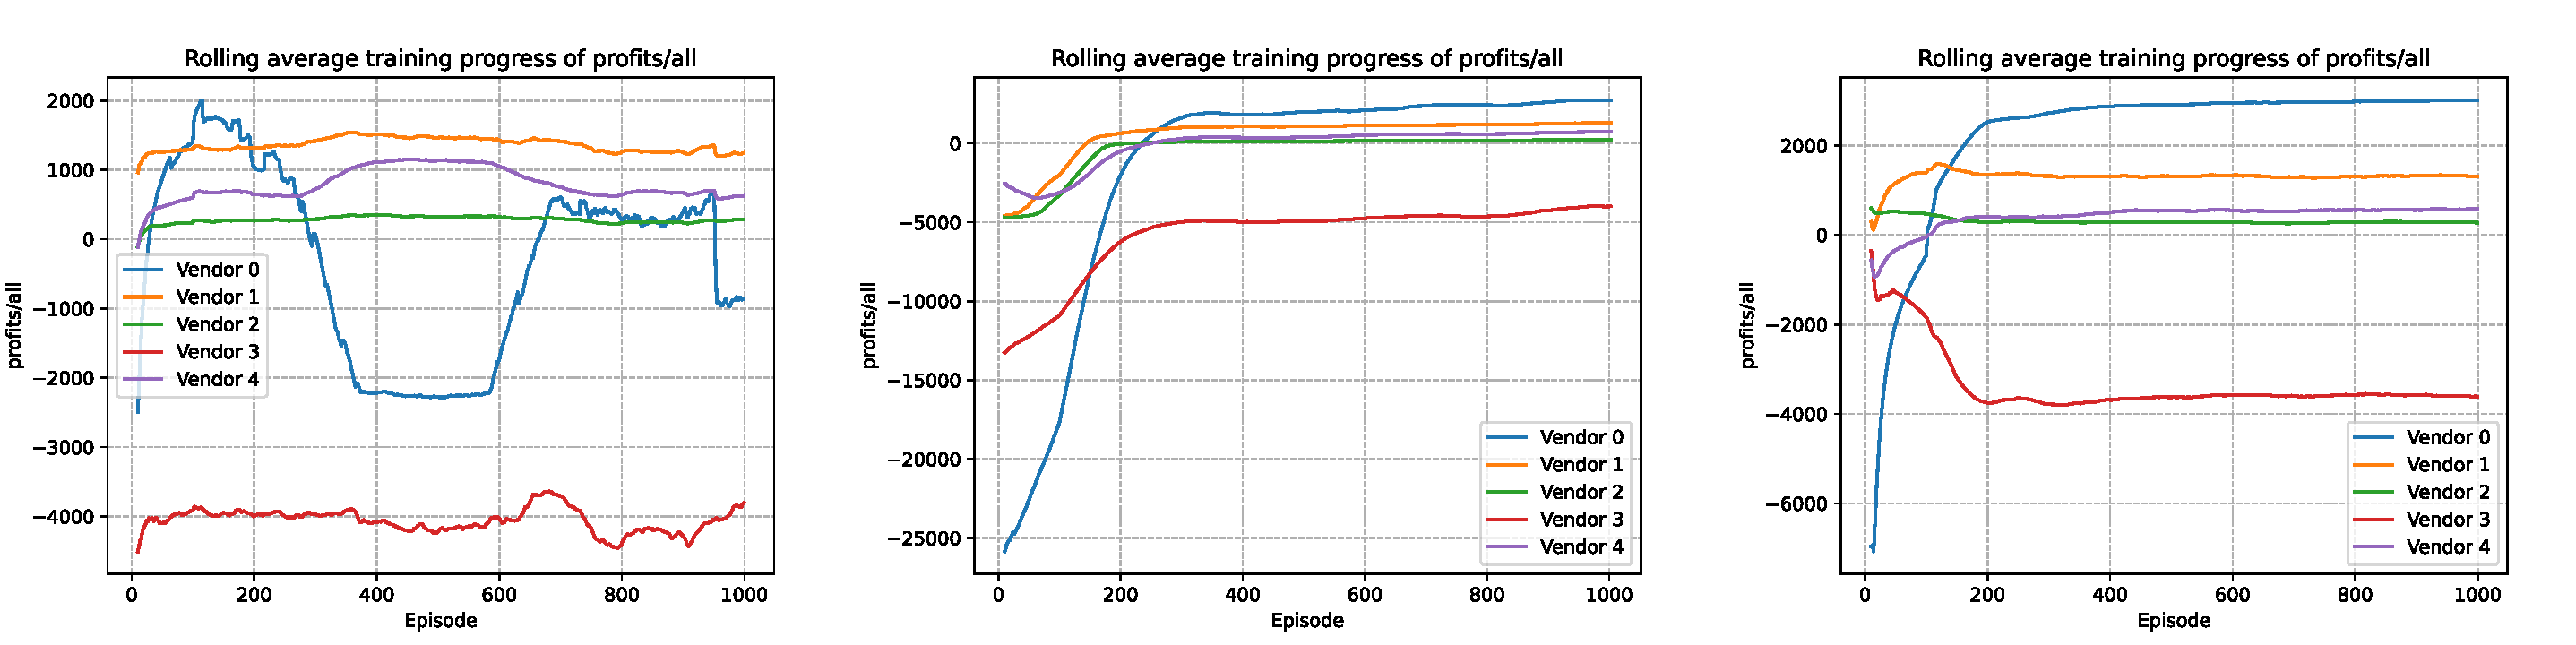
\includegraphics[width=\textwidth]{main/oligopoly_vendor_comparison.pdf}
	\caption{Profite typischer Trainingsdurchläufe von A2C, PPO und SAC im Vergleich zu ihren regelbasierten Konkurrenten}
	\label{graphic:OligopolyVendorComparison}
\end{figure}

Abbildung \ref{graphic:OligopolyVendorComparison} zeigt für jeden der drei Algorithmen einen typischen Trainingsdurchlauf.
Die Ergebnisse sind dabei äußerst zufriedenstellend.
Jeder der RL-Agenten kann während seines Trainingsdurchlaufes alle seine regelbasierten Konkurrenten deutlich übertreffen.
Der Agent mit den festen Preisen schneidet erwartungsgemäß am schlechtesten ab, da er weder dazu in der Lage ist, sein Lager zu regulieren, noch auf Preise der Konkurrenten zu reagieren.
Der Agent, der nur sein Lager reguliert, landet auf dem vorletzten Platz, während die beiden regelbasierten Agenten, die auch auf Konkurrenzpreise reagieren, passabel abschneiden.

In diesem Oligopolszenario tritt der Effekt, dass ein RL-Agent einen regelbasierten Konkurrenten überholen lässt, nicht auf.
Weil die RL-Agenten ihre Konkurrenz hier stets überholen, besteht nicht die Notwendigkeit für die gemischte Rewardfunktion.
Deshalb werden diese Versuche auch nicht detailliert betrachtet.

Für echte Märkte mit mehreren Anbietern und höherdimensionalen Beobachtungen ist es eine sehr wichtige Erkenntnis, dass auch dieses kompliziertere Szenario durch die RL-Algorithmen mit einer gewissen Lässigkeit und äußerst zuverlässig gelöst werden kann.
Das unterstreicht die praktische Anwendbarkeit von RL-Algorithmen auf Marktplätzen.